\documentclass[12pt]{article}
\usepackage{amsmath, amsthm, amssymb}
\usepackage{float}
\usepackage{rotating}
\usepackage{graphicx} 
%\usepackage{subfig} 
\usepackage{longtable} 
\usepackage{xcolor}
\usepackage[colorlinks=true, urlcolor=cyan, linkcolor=olive]{hyperref}
\usepackage[margin=1in]{geometry}
\usepackage[font=small,format=plain,labelfont=bf,up,textfont=it,up]{caption}
\usepackage{subfig}
\usepackage[utf8]{inputenc}
\usepackage[utf8]{inputenc}
\usepackage[T1]{fontenc}
\usepackage{fixltx2e}
\usepackage{graphicx}
\usepackage{float}
\usepackage{wrapfig}
\usepackage{soul}
\usepackage{textcomp}
\usepackage{marvosym}
\usepackage{wasysym}
\usepackage{latexsym}
\usepackage{amssymb}
\usepackage{hyperref}
\usepackage{multirow}
\usepackage{pdflscape}  
\tolerance=1000
\usepackage{color}
\usepackage{listings}
\lstset{
language=R,
keywordstyle=\color{blue!75!black},
commentstyle=\color{red!75!black},
stringstyle=\color{green!75!black},
basicstyle=\ttfamily\footnotesize,
columns=fullflexible,
tabsize=4,
backgroundcolor=\color{white!95!black},
basewidth={0.5em,0.4em}
}
\RequirePackage{fancyvrb}
\DefineVerbatimEnvironment{verbatim}{Verbatim}{fontsize=\small,formatcom={\color[rgb]{0.5,0,0}}}
\newtheorem{example}{Example}
\newtheorem{definition}{Definition}
\newtheorem{proposition}{Proposition}
\newtheorem{remark}{Remark}
\newtheorem{conjecture}{Conjecture}
\newtheorem{lemma}{Lemma}
\providecommand{\alert}[1]{\textbf{#1}}
\begin{document}

\title{Ambiguity, Learning and Insurance}
\author{Anmol Bhandari \thanks{Economics Department; New York University \texttt{apb296@nyu.edu}}}
%\date{03 March 2011}
\maketitle
I study  optimal risk sharing in settings characterized with Knightian uncertainty. In general there is a feedback between risk sharing and risk perceptions which impacts the optimal risk sharing arrangement. This paper attempts to identify the key mechanisms affecting insurance in \emph{stylized} environments differing in two dimensions - market completeness and nature of ambiguity
\newpage

\section{Introduction}
\noindent General equilibrium with complete markets provide a coherent framework to explore risk sharing amongst competitive agents. Attitudes towards risk and class of securities available are the key objects for determining a risk sharing arrangement. The welfare theorems in turn justify the \emph{optimality} of such arrangements. The standard analysis with Von-Neumann preferences,complete information and appropriate selection of assets has very stark predictions for the optimal risk sharing scheme. All idiosyncratic risk is hedged and aggregate risk is borne by the agents depending on their initial wealth distribution. With homothetic preferences we further have consumption as a constant proportion of aggregate endowment and wealth distribution is static. 

\vspace{3mm}
With incomplete markets agents can \emph{self-insure} some of the idiosyncratic risk. The extent of insurance then depdens on how incomplete the asset markets are. In case of endogenously incomplete markets incentives constraints are key in affecting the level of insurance.

\noindent In this paper I explore the qualitative differences in the optimal risk sharing schemes where the distinction between risk and uncertainty is explicit. The settings will differ in two dimensions  - nature of market completeness and nature of ambiguity. 

%% CHECK THE PACKAGE FOR COLUMNS

%\vspace{4mm}
%\begin{columns}
%  \begin{column}{0.5\textwidth}
%  \textbf{Market structure}
%    \begin{itemize}
%\item \small Complete markets 
%	\item  \small Exogenously incomplete markets - Bond economy
%	\item \small  Endogenously incomplete markets - Private information frictions
%   \end{itemize}
%  \end{column}
%  \begin{column}{0.5\textwidth}
%  \textbf{Ambiguity}
%     \begin{itemize}
%     \item[]
%\item \small  Uncertainty about endowment shocks  (observable)
%\item \small  Uncertainty about parameters ( or regimes) (unobservable)
%     \end{itemize}
%  \end{column}
%\end{columns}


\section{Key Results}
\noindent The basic mechanism studied is the interplay between insurance and pessimism in a general equilibrium framework. Ex-ante identical agents may be subject to different continuation trajectories depending how idiosyncratic and aggregate risk/uncertainty is resolved in equilibrium. These different continuation trajectories will imply that agents who fear model uncertainty will choose different decision rules including how they learn about the parameters.

\noindent In the complete market setting model with aggregate randomness , uncertainty results in consumption shares depending on realizations of aggregate endowment. When utility is bounded from below wealthy agents who bear most of the aggregate risk over-insure themselves in low endowment states. Further in type (II) ambiguity qualitatively changes the risk sharing arrangement.With parameter uncertainty, consumption shares depend on realization of idiosyncratic endowments due to asymmetric reduction of compound lotteries. This has implications for asset prices and long-term survival. Market price of risk now depends on the relative wealth differences and is higher at the extremes. Further  the fact that agents beliefs (ex-post) diverge from their reference models depending on their wealth affects long run survival. In particular this generates survival possibilities for small perturbations from the correct reference model. This is in stark contrast with expected utility case where arbitrarily small 
perturbations can cause such agents vanish asymptotically. 

Market incompleteness introduces the prospect of un-insurable idiosyncratic risk. Now agents with higher wealth levels are relatively optimistic about their income distribution. The key force here is \emph{self-insurance}. Having a large amount of wealth reduces the randomness and concerns for misspecification for wealthy agents. This force survives the setting when markets are endogenously incomplete. To this end, I study a simple case where private information frictions affect the extent of risk-sharing. On one hand relative differences in beliefs requires consumption shares to be tilted towards agents who perceive the state more likely. However the extent to which this can be done depends on the incentives (truth-telling) constraints. Overall both these restrictions shape the insurance arrangement.

\section{Preferences towards Knightian uncertainty}
\noindent Knightian uncertainty in this context refers to an environment where risk cannot be perfectly quantified by an an agent. A specific source of Knightian uncertainty is the statistical closeness of different models of risk. \footnote{By ``model of risk' - I refer to a probability measure over future contingencies}.A feature common to any model of Knightian uncertainty as against a Bayesian benchmark is the presence of multiple priors and a rule describing how the decision maker selects a relevant prior. To complete a description of how agents behave in this setting we must specify a theory of how they deal with this multiplicity. Most models of ambiguity \footnote{refer to a subset of papers } try to recast the decision making problem by positing a prior selection rule confirming certain behavioral regularities. This prior selection rule opens up c channel of linking `ex-post' beliefs to other endogenous aspects of the environment. In this paper I follow Hansen Sargent (2007) version of recursive 
multiplier preferences. With these preferences the decision maker confronts alternative models of risk by following a \textbf{\emph{robust}} approach. In particular he makes use of an hypothetical `malevolent agent' to design decision rules that are robust to the potential misspecification he is worried about. 

\noindent A recurring theme in the formulation of ``statistical closeness'' will be the notion of ``Relative Entropy''. \footnote{This is also referred to the \emph{Kullback-Leiblar divergence} . It arises as the exponent of the probability error in an hypothesis test between two distributions}
\begin{definition}
Consider two P and Q two absolutely continuous measures over a set X, the relative entropy between P, and Q is defined as 
\[\mathcal{E}_{P,Q} = \int_{X}\log\frac{{dP}}{dQ}dP\]
Let $m=\frac{{dP}}{dQ}$, we can write the above as $\mathbb{E}_Q [m \log m]$
\end{definition}

There are two related ways of formalizing the robust approach under the fear of model misspecification. 
\begin{enumerate}
	\item Multiplier Preferences : \[\max_{a}\min_{m\geq 0; \mathbb{E}m=1} \mathbb{E}m\{V(X,a) + \theta \log m \}\]
	\item Constraint Preferences : \[\max_{a}\min_{m\geq 0; \mathbb{E}m=1} \mathbb{E}\{V(X,a) \}\]
	s.t 
	\[\mathbb{E}m\log m \leq \eta\]
	
\end{enumerate}
The minimization in both the problem reflects the misspecification fears. In some sense the agent explores set a models in the vicinity of a reference model penalized by $\theta$ (or the controlled by $\eta$) to make sure he optimizes in the worst case scenario. In the next few section I will use the generalization of the multiplier preferences to incorporate dynamic ambiguity and learning as in Hansen Sargent (2007).
	
\section{Static Example - Risk Sharing and Risk Perceptions}
A new mechanism present in models of Knightian uncertainty is the link between risk sharing and risk perceptions. A risk sharing scheme is a state contingent plan of outcomes for an agent. As mentioned earlier, the agent uses his utility outcomes to various models as an input for decision-making, in particular selecting a relevant model of risk which rationalizes his actions. Thus how risk is shared affects what prior gets selected, but this in turn affects how much an agent is prepared to pay for the insurance. We can see one part of the link in a very simplified static example as below.
\vspace{10 mm}

\noindent Let $Y(z)$ be a risky endowment to be shared amongst $K$ agents who value consumption by $u(c)=\frac{c^{1-\gamma}}{1-\gamma}$. Denote $p(y)$ as the density of $Y$ over its support $[\underline{Y} \quad \bar{Y}]$

\noindent  Denote a feasible risk sharing arrangement by $\alpha = [\alpha_1 \dots \alpha_K]$ such that $\sum \alpha_i=1$

\noindent  Now suppose that the agents do not trust the distribution of $Y$ but have a common approximating model $p(y)$ and are using the multiplier version of the model

\[V^R (\alpha_i)=\min_{m \geq0;\mathbb{E}m=1}\mathbb{E}m[u(\alpha_iY)+\theta\log(m)]\]

\noindent  The choice for $m^*$ which solves this problem is

\[m_i^*\propto \exp\left\{\frac {-\alpha^{1-\gamma}_iy^{1-\gamma}}{\theta(1-\gamma)}\right\}\]

\noindent An ex-post Bayesian interpretation : Agents have (diverse) priors given by $\tilde{p}_i(y)=p(y)m^*_i(y)$. 

\noindent  The following proposition shows how the relative pessimism depdens on $\alpha_i$

\begin{proposition}
\label{propo-1}
\begin{enumerate}
	\item $\lim_{\alpha_i \to 0} \tilde{p}_i(\underline{Y})=p(\underline{Y}) \quad \gamma < 1$
	\item $\lim_{\alpha_i \to 0} \tilde{p}_i^*(\underline{Y})=1  \quad \gamma > 1$
\end{enumerate}
\end{proposition}
\begin{proof}
\[m^*_i(y)=\frac{\exp\left\{\frac {-\alpha^{1-\gamma}_iy^{1-\gamma}}{\theta(1-\gamma)}\right\} }{\mathbb{E}\exp\left\{\frac {-\alpha^{1-\gamma}_iy^{1-\gamma}}{\theta(1-\gamma)}\right\} }\]

Note that at $y=\underline{Y}$
\[\frac{\partial \log m_i(\underline{Y}) }{\alpha_i} = \frac{\alpha^{-\gamma}}{\theta}\left[ \tilde{\mathbb{E}} y^{1-\gamma} -\underline{Y}^{1-\gamma}\right]\]
Since $\underline {Y} $ is the lower end of the support, we have the term on the RHS of the above derivative to be positive iff $\gamma < 1$ Thus we have two porperties,
	\begin{itemize}
          \item $\tilde{p}_i(y) < p(y) \forall y$
          \item $\lim_{\alpha_i \to 0} \tilde{p}_i(\underline{Y})=1$
         \end{itemize}

With $\gamma > 1$, however, $\tilde{p}_i(\underline{Y})$ increases as $\alpha_i$ approaches 0, and \footnote{$\gamma > 1$, $m^*_i$ is not defined at $\alpha_i=0$ as the utility is unbounded in that case.} 
\[\lim_{\alpha_i \to 0}\tilde{p}_i(\underline{Y}) = 1\]



\end{proof}


\noindent  This roughly means that agents with low shares of aggregate endowmwnt are realtively more optimistic when the there is a lower bound on the utility. With $\gamma < 1$, we have a natural lower bound on utility i.e 0. With $\gamma > 1$ utility diverges to $\infty$ as cosumption goes to zero. This highlights the forces that will affect relative beliefs as wealth shares move around. Also the distiction between $\gamma$ less than and greater than one plays an important role in the survival analysis discussed later

\vspace{10 mm}
\noindent Now in a general equilibrium setup- agents this interplay will affect the demand for insurance and optimal risk sharing.In particular ex-ante identical guys may be subject to different continuation trajectories depending how idiosyncratic and aggregate risk/uncertainty is resolved in equilibrium. These different continuation trajectories will imply that ambiguity averse agents who fear for the worst model will choose different decision rules including how they learn about hidden state variables.

Note that this depends on $\alpha$ as long as $\gamma\neq 1$. As will be shown later $\gamma=1$ case boils down to the special case of Epstien-Zin preferences. The homotheticity properties of these preference imply that in absence of preference heterogenity the risk sharing scheme is independent of concerns for model ambiguity as long as markets are complete



\noindent In most of my discussion I will use $\gamma < 1$. As explained later this has useful stability properties for wealth shares. Although a realistic calibration of paramters is beyond the scope of the paper, a natural question arises whether $\gamma < 1$ restrictive. Note that under the version of static multiplier preferences as above, attitudes towards randomness are captured by jointly by two parameters : $\theta, \gamma$. Hence the typical interpretation of $\gamma$ as the coeffecients of relative risk aversion in the benchmark case is lost. The following heuritic example makes the point more clear. 

\noindent \emph{Consider a thought experiment. An agent starts with wealth $W$ is confronted with a lottery of gaining or loosing $\kappa W$ with probability $(p,1-p)$. Let $\mathbb{C}[\theta,\gamma|W,\kappa]$ be the ambiguity adjusted certainty equivalent defined in the usual sense}
\[
\mathbb{C}[\theta,\gamma|W,\kappa] : \frac { (W-c)^{1-\gamma} } {1-\gamma}=
-\theta \log
\left(
p \exp\left \{-\frac {[W(1+\kappa)]^{1-\gamma}}  {\theta (1-\gamma)} \right \}
+(1-p)\exp \left \{-\frac {[W(1-\kappa)]^{1-\gamma}} {\theta (1-\gamma)} \right\} \right)\]

\noindent Figure \ref{fig:CertaintyEq} plots the level curves for $\mathbb{C}[\theta,\gamma|W,\kappa]$. The level curves are relatively flat with respect to $\gamma$ at low values of $\theta$ and then eventually become steeper with $\theta$ approaching the expected utility levels. Thus  high values of $\gamma$ can be substituted for low values of $\theta$ keeping the certainty eqvivalent fixed. 

\begin{figure}[htbp]
\centering
\includegraphics[scale=.75]{Matlab/CertaintyEq.png}
\caption{This figure level curve for the $\mathbb{C}[\theta,\gamma]$ for $W=1,\kappa=\frac{1}{10}, p=\frac{1}{2}$.}
\label{fig:CertaintyEq}
\end{figure}




\vspace{10 mm}
\noindent  A further observation is that this mechanism has a space for \emph{endogenous} emergence of heterogeneous beliefs. This route of belief heterogeneity is very different from the ones usually resorted in theory, namely
\begin{enumerate}
	\item Exogenous  - Harrison and Kreps
	\item Asymmetric Information : Grossman Stiglitz
	\item Rational Inattention  : Sims
\end{enumerate}

\noindent Here agents with symmetric information may `choose' to have different beliefs because their continuation values vary differently. More importantly this theory of heterogenous beliefs is tied down with equilibrium objects and is potentially testable through over-identifying restrictions.

\section{Model}
In this section I will specify the key ingredients of the setup for the complete markets environment. Both the exogenous and endogenous incomplete markets will modify this setup.
\subsection{Setup}
\begin{enumerate}
		\item \textbf{Agents}  : $I$ is the  set of agents, where $I= \{1,2\}$
		\item \textbf{Technology} : Exchange economy
		\item \textbf{Endowments}  : Two Shocks - Size and
                  Distribution of aggregate endowment - $z=(y,s)$

									\begin{itemize}
											\item $M$ be the cardinality of the Model Space
											\item $\mathcal{M}=\{\alpha_m,\beta_m\}_{m\leq M}$ is the Model Space
									\end{itemize}
									
\noindent Given a model we have $P(z^*|z,m)=\mathbb{P}_{Z}[\alpha_m,\beta_m]$. We can have the model space evolving (like regime changes) as a Markov process $\{\mathcal{M},\mathbb{P}_{M},\pi^0_{M}\}$ \footnote{This allows me interpret type (II) ambiguity as concerns for unknow parameters when $P_M=\mathbb{I}$ and regimes otherwise.}. With this setup we have the following state-space

\[m_{t+1} | m_t \sim \mathbb{P}_{M}\]
\[z_{t+1}|z_t,m_t \sim \mathbb{P}_{Z}(\alpha_{m_t},\beta_{m_t})\]

\item \textbf{Preferences} : Following Hansen and Sargent [2007] the preferences of the agent are described by 2 sets of 		objects, 
								\begin{itemize}
										\item \textbf{Ambiguity}
													$\forall i \in I,$
												\begin{enumerate}
															\item Approximating Models :   $\left\langle  P^i_M,P_Z^i, \pi^i \right\rangle$
															\item Entropy Penalty - $\theta_j^i$ where $j=2$ captures the doubts about the parameter $m$ and $j=1$ about the $z^*$ given $z$
												\end{enumerate}
											\item \textbf{Time and Risk} :
																\begin{enumerate}
																		\item Risk Aversion - $\gamma^i$
																		\item Subjective discount factor - $\delta^i$
																\end{enumerate}
 												\end{itemize}
\end{enumerate}
The agents can have potentially different preferences but I will mostly concentrate on the cases where the only differences in the agent is their endowment stream. Given the model $\alpha_m=\alpha$ and $\beta_m= \beta$ the transition matrix $\mathbb{P}_{Z}$ is constructed as below. 

\begin{equation}
\label{mat:Pz}
P_Z(z^*|z,m)=P_{Y} (y^*|y,\alpha_m)P_{S|Y} (s^*|y^*,\beta (y^*)) 
\end{equation}

\[P_Y=\bordermatrix{\text{}y_l&y_h\cr
                y_l&\alpha  & (1-\alpha)\cr
                y_h&   (1-\alpha) &   \alpha(1-\beta)}\]
                
\[P_{S|Y}=\bordermatrix{\text{}&s_l&s_h\cr
                y_l& \beta^l & (1-\beta^l)\cr
                y_h&   \beta^h & (1-\beta^h)}\]
                
Note that $\beta$ is a vector of the same dimension as the dimension of the aggregate endowment shock.

\footnote{With this choice I allow for $s$,$y$ to be correlated but $s$ does not \emph{Granger} cause $y$. This choice can be relaxed but will be useful for \ref{propo-5}}

%\[P_Z=\bordermatrix{\text{}&y_ls_l&y_ls_h&y_hs_l&y_hs_h\cr
%                y_ls_l&\alpha\beta&  \alpha(1-\beta)  & (1-\alpha)\beta& (1-\alpha)(1-\beta)\cr
%                y_ls_h&   \alpha(1-\beta) &  \alpha\beta &(1-\alpha)(1-\beta) & (1-\alpha)\beta\cr
%                y_hs_l&   (1-\alpha)(\beta) &  (1-\alpha)(1-\beta )&\alpha\beta & \alpha(1-\beta)\cr
%                y_hs_h&  (1-\alpha)(1-\beta) &  (1-\alpha)\beta &\alpha(1-\beta) & \alpha\beta }\]
%


\subsubsection{Dynamic Ambiguity and Learning}
\label{sec:Dynamic-Amb-Learning}
In this section, I will briefly summarize how to extend the static multiplier version of these preferences to incorporate dynamics under different information structures. At first it might seem a separation argument should make these things independent-In particular how an agent filters payoff relevant hidden states and how he evaluates \emph{ risky consumption streams} should not be related. This is indeed true in a Bayesian framework, where learning/filtering is dictated by applying some form of Bayes rule. In simple words the agent has a prior, observes signals , updates his posterior and evaluates risk with those posteriors. However with multiple priors, future utility consequences may induce the agent to re-evaluate the past learning outcomes. In particular this introduces two sources of misspecification conceptually similar to compound lotteries. The agent may mistrust his prior over hidden states and/or the transition density governing the future signal/state evolution given the  hidden state. Hansen 
Sargent (2005),Hansen Sargent (2007) take two separate stands on how the agent treats past distortions. In Hansen Sargent (2005), the agent is committed to past misspecifications, which means that the reference prior in any period inherits the past distortions to priors. In Hansen Sargent (2007), they formulate the problem without commitment,which means the agent's reference prior in any period consists of the relevant Bayesian updated prior under his approximating model. Once we obtain the relevant prior either with or without commitment, the agent expresses is distrust by applying two operators - $\mathbb{T}_1$ and $\mathbb{T}_2$  described as follows.

I will focus on the ``no-committment'' version henceforth. This assumption implies that the agent distrusts the outcome of learnng rather than the process. Mechanically he applyes Bayes Rule to update his posteriors over $m_t$ and at each point evaluates across model utility consequences to distort this Bayes posterior. 


\noindent Let $X_t=[Z_t \quad M_t]'$ where $X_t$ is the state variable with $Z_t$ as the observable part and $M_t$ as the unobservable part. Denote $\mathcal{X}_t = \sigma(X^t)$, $\mathcal{Z}_t=\sigma(Z^t)$ as the sigma algebras generated by $\{X_i\}^{t}_{i=0}$ and $\{Z_i\}^{t}_{i=0}$ respectively. 

\begin{definition}	
Operator $\mathbb{T}^1_{\theta_1,t} : \mathcal{L}^2(\mathcal{X}_{t}) \to \mathcal{L}^2(\mathcal{X}_{t+1}) $ is given by
\[\mathbb{T}^1_t[W_{t+1}] = \min_{m_{t+1}; \mathbb{E}m_{t+1}=1} \mathbb{E}\left[m_{t+1}\left( W_{t+1} +\theta_1 \log(m_{t+1})\right)| \mathcal{X}_t\right] \]
\end{definition}
\noindent Similarly, 
\begin{definition}
Operator $\mathbb{T}^2_{\theta_2,t} : \mathcal{L}^2(\mathcal{X}_{t}) \to \mathcal{L}^2(\mathcal{S}_t) $ is given by
\[\mathbb{T}^2_t[\hat{W}_t] = \min_{h_{t}; \mathbb{E}h_t=1} \mathbb{E}\left[h_{t}\left( \hat{W}_t +\theta_2 \log(h_{t})\right)| \mathcal{S}_t\right] \]
\end{definition}
\footnote{$\mathbb{E}$ refers to expectations under the relevant approximating model}
This notation allows us to write the preferences of the agent as follows. Given a stochastic process for consumtption given by $c(z)$ we have 
\[\mathcal{Q}_c(\pi,z)=\mathbb{T}^2_{\theta_2}\left[u(c(z))+\delta\mathbb{T}^1_{\theta_1,m} \mathcal{Q}_c^*(\pi^*,z^*)\right]\]
where

\[z^*|z \sim P_Z(z^*|z,m)\]
\[\pi^{*}(m^*)\propto \sum_{m}{\pi(m) P_Z(z^*|z,m)P_M(m^*}|m)\]





\section{Planner's Problem}
In this section, I setup the recursive planner's problem in the `Dynamic programing squared' tradition where continuation values are state variables. This formulation is convenient for when private information frictions are introduced. The solution to this problem characterizes all effecient allocations. Appendix A shows the equivalence between the planner's problem and the decentralized competitive equilibria. The planner distributes the risky aggregate endowment between the two agents in a way that he meets the promised ex-ante present discounted value of utility to agent 2 and maximizes the welfare of agent 1. With uncertainty, a given consumption plan alters the beliefs of the agents and thus expected value of the stream. Thus at the margin, while equating  probability weighted marginal utilities across agents and time, the Planner realizes that new force of endogenous beliefs. This manifests itself as time varying continuation values or Pareto weights.

\noindent  Let z=(y,s) summarize the states

\noindent $\mathcal{Q}(v,z,\pi)$ be the maximum lifetime discounted utility of agent 1 given that $v$ is the promised lifetime discounted utility of agent 2.
\begin{equation}
\mathcal{Q}(v,z,\pi)=\max_{c,v^*(z^*)} \mathbb{T}_2\left[u^1(c)+\delta \mathbb{T}_1 \mathcal{Q}(v^*,z^*,\pi^*)\right]
\label{eq:PP}
\end{equation}
\begin{subequations}
\begin{equation}
\label{eq:PK}
\mathbb{T}_2\left[u^2(y-c)+\delta \mathbb{T}_1 v^*\right]\geq v
\end{equation}
\begin{equation}
\pi^{*}(m^*)\propto \sum_{m}{\pi(m) P_Z(z^*|z,m)P_M(m^{*}|m)}
\end{equation}
\end{subequations}
\begin{remark}
This conveniently extends to more than 2 agents. We would need to keep track of promises to all the agents and have a \ref{eq:PK} for each of the agent except Agent 1.
\end{remark}
\subsection{Analysis of the Planner's problem}
 Let $\lambda$ be the multiplier associated with the promise-keeping constraint, the F.O.C characterizing the solution to the Planner's problem are as follows,
 \begin{subequations}
\begin{equation}
u^1_c(c)=\lambda u^2_c(y-c)
\label{eq:FOC_c}
\end{equation}

\begin{equation}
\left(\sum_{m \in M}\tilde{\pi}^1(m)\tilde{P^1}_z(z^* |z,m)\right)\lambda^*=\lambda\left(\sum_{m \in M}\tilde{\pi}^2(m)\tilde{P^2}_z(z^* |z,m)\right) 
\label{eq:FOC_vstar}
\end{equation}
\end{subequations}

\begin{subequations}
\begin{align}
\tilde{P}^1 & \propto P\exp\left\{\frac{-\mathcal{Q}(v^*,z^*,\pi^*)}{\theta^1}\right\}\\
\tilde{P}^2 & \propto P\exp\left\{\frac{-v^*}{\theta^1}\right\}\\
\tilde{\pi}^1 & \propto \pi \exp\left\{-\frac{ u^1(c)+\delta \mathbb{T}^1_2 \mathcal{Q}(v^*,z^*,\pi^*) }{\theta^2}\right\} 
\end{align}
\end{subequations}

 
 
Consider the Lagrangian for the Planner's problem
\[\mathcal{L}(v,z,\pi,\lambda) = \left(\mathbb{T}_2\left[u^1(c)+\delta \mathbb{T}_1 \mathcal{Q}(v^*,z^*,\pi^*)\right]\right)+\lambda(\mathbb{T}_2\left[u^2(y-c)+\delta \mathbb{T}_1 v^*\right]-v)\]
The multiplier $\lambda$ plays the role of the traditional relative ``Pareto weights''. 

\noindent We have a mapping between $\lambda$ and $v$ given by the Envelope theorem
\[\lambda=-\mathcal{Q}_v(v,z,\pi)\]

\noindent Equation (2) captures the Planner's key inter temporal trade offs. In a standard case with Expected Utility, we would have 
\[\lambda_{EU}^*=\lambda_{EU}\]
\begin{remark}
The first order conditions reveal that the allocations in this economy would be equivalent to an economy with $\theta_1,\theta_2=\infty$ and exogenous (heterogenous) beliefs which are equivalent to the worst case beleifs of this model. This mapping allows us to analyze this economy as a combination of a standard heterogenous beleif expected utility risk sharing problem plus a theory of how these beleifs are pinned down. 
\end{remark}
\begin{remark}
Anderson (2005) formulates the recursive problem using Pareto weights as the state varaibles. This maps into the current problem by recognizing that the envelope theorem links the $v$ and $\lambda$
\end{remark}
\section{Insurance Arrangements  - Complete Market}




Further define $v^{max}(z,\pi)$ and $\bar{v}(z,\pi)$ as follows
\[v^{max}(z,\pi)=\mathbb{T}^2_{\theta_2}[u(y)+\delta \mathbb{T}^1_{\theta_1,m}v^{max}(z^*,\pi^*)]\]

\[\bar{v}(z,\pi) : Q[\bar{v},z,\pi]=\bar{v}\]
\begin{proposition}
\label{propo-2}
If $v=\bar{v}$, 
\begin{enumerate}
	\item $v^*(z^* |z,\bar{v},\pi) = \bar{v}(z^*,\pi^*)$
	\item $c(v,z,\pi)=\frac{y(z)}{2}$
\end{enumerate}
\end{proposition}
\begin{proof}
The definition of $\bar{v}$ implies that 
\[Q_v(\bar{v},z,\pi)=-\lambda=1\]

Thus from the FOC with respect to $c$ we have $c(\bar{v},z,\pi)=\frac{y(z)}{2}$. Now we check whether the guessed policy for $v^*(z^*|\bar{v},z,\pi)$ solves the FOC and the PK constraint.

\noindent First we have that $\lambda^*=1$ and since the utility consequences for both the agents are identical $Q^*=v^*$ they distort the underlying models in the same way. Thus the other FOCs are satisfied. Lastly the PK constraint is met as follows
\[\mathcal{Q}(\bar{v},z,\pi)=\max_{c,v^*(z^*)} \mathbb{T}_2\left[u^1(c)+\delta \mathbb{T}_1 \mathcal{Q}(v^*,z^*,\pi^*)\right]\]
\[\mathcal{Q}(\bar{v},z,\pi)=\mathbb{T}_2\left[u^1(\frac{y(z)}{2})+\delta \mathbb{T}_1 \mathcal{Q}(\bar{v}^*,z^*,\pi^*)\right]\]
\[\mathcal{Q}(\bar{v},z,\pi)=\mathbb{T}_2\left[u^1(\frac{y(z)}{2})+\delta \mathbb{T}_1 \bar{v}^*\right]\]
\[\bar{v}(z,\pi)=\mathbb{T}_2\left[u^1(y-c(\bar{v},z,\pi))+\delta \mathbb{T}_1 v^*\right]\]
\end{proof}

The choice for intial promised value $v=\bar{v}$ correspond to what Anderson (2005) referred to as $\emph{steady states}$ modified for presence of hidden states. The intuition behind these is that the setup collapses to a representative agent economy with an appropiate choice of initial wealth distribution. The only differences amongs the agent I am focusing on is coming from initial wealth heterogenity. Given a choice for idiosyncratic endowments there exists a intial distribution of wealth such that this heterogenity is eliminated. Proposition \ref{propo-1} further specifies that begining from such a point the economy stays there always
\begin{proposition}

The next proposition isolated two special cases where the risk sharing arrangement is indepdent of the ambiguity paramters $\theta_1$ and $\theta_2$
\label{propo-2}
With $\gamma=1$ or $y_{l}=y_{h}$, the risk sharing scheme is independent of $\theta_1$ and $\theta_2$
\end{proposition}
\begin{proof}

\noindent Define $V_{\alpha}(z,\pi)$ as the value of consuming a fixed share $\alpha$ of the aggregate endowment. With $\gamma=1$ we can compute $V_{\alpha}$ in closed form. 

\noindent Guess $V_{\alpha}(z,\pi) = \mathcal{L}_0(z,\pi)+\mathcal{L}_1 \log{ \alpha}$. We can now pin down the unknown function $\mathcal{L}_0$ and the constant $\mathcal{L}_1$ with the following Bellman equation
\begin{equation}
V_{\alpha}(z,\pi)=\mathbb{T}^2_{\theta_2}\left[\log[\alpha y(z)]+\delta \mathbb{T}^1_{\theta_1,m} V_{\alpha}(z^*,\pi^*)\right]
\end{equation}

First we apply the $\mathbb{T}^1_{\theta,m}$ operator,
\begin{align*}
\mathbb{T}_{\theta_1,m} V_{\alpha}(z^*,\pi^*)&=& -\theta_1 \log \sum_{z^*}{\exp\left\{ \frac{-V_{\alpha}(z^*,\pi^*)}{\theta_1}\right\}P_Z(z^*|z,m)} \\
&=& \mathcal{L}_1 \log(\alpha) -\theta_1 \log \sum_{z^*}{\exp\left\{ \frac{-\mathcal{L}_0(z^*,\pi^*)}{\theta_1}\right\}P_Z(z^*|z,m)} \\
%\mathbb{T}_{\theta_1,m} V_{\alpha}[z^*,\pi^*]&=& \mathcal{L}_1\log(\alpha)-\theta_1 \log \sum_{z^*}{\exp\left\{ \frac{-V_{1}[z^*,\pi^*]}{\theta_1}\right\}P_Z(z^*|z,m)} \\
\end{align*}
\noindent  Similiarly after applying the $\mathbb{T}^2_{\theta_2}$ operator we have

\begin{equation}
V_{\alpha}(z,\pi)=(1+\delta \mathcal{L}_1)\log(\alpha)+ \log[y(z)] + \mathbb{T}^2_{\theta_2} \left[-\theta_1 \delta \log \sum_{z^*}{\exp\left\{ \frac{-\mathcal{L}_0(z^*,\pi^*)}{\theta_1}\right\}P_Z(z^*|z,m)}\right]
\end{equation}

\noindent Mathcing coeffecients we have
\begin{subequations}
\begin{equation}
\mathcal{L}_1 =\frac{1}{1-\delta}
\end{equation}

\begin{equation}
\mathcal{L}_0(z,\pi) = \log[y(z)] + \mathbb{T}^2_{\theta_2} \left[-\theta_1 \delta \log \sum_{z^*}{\exp\left\{ \frac{-\mathcal{L}_0(z^*,\pi^*)}{\theta_1}\right\}P_Z(z^*|z,m)}\right] \quad \forall \quad z,\pi
\end{equation}
\end{subequations}

\noindent  Next we define $\alpha (v,z, \pi)$ as 

\[V_{\alpha(v,z,\pi)}=v\], using the guess for $V_{\alpha}$ we can show that

\begin{equation}
\alpha (v,z,\pi) = \exp \{ \frac{v-\mathcal{L}_0 [z,\pi]}{ \mathcal{L}_1}\}
\label{eq:alphadef}
\end{equation}


\noindent  Finally we check that $Q(v,z,\pi) = V_{1-\alpha(v,z,\pi)} (z,\pi)$ solves the Planner's problem with the following policy rules

\[c(v,z,\pi)=\alpha (v,z,\pi) y(z)\]
and
\[v^* (z^* | v,z,\pi) = V_{\alpha (z,\pi,v)} [z^*,\pi^*(z^*,\pi,z)]\]

Where $\pi^*$ is given by Bayes Law

\noindent Note that the PK is satisfied by these policy functions. The envelope theorem implies that 
\[\lambda (v,z\pi) = -\frac{\partial Q (v,z,pi)}{\partial v}\]
or 
\begin{equation}
\lambda (v,z\pi) = -\frac{\mathcal{L}_1 \alpha_v(z,\pi,v)}{1-\alpha (v,z,\pi)}
\label{eq:lambda}
\end{equation}

Since $\alpha_v(v,z,\pi) = -\frac{\alpha (v,z,pi)}{\mathcal{L}_1}$ we can verify the FOC with respect to $c$ is satisfied


\noindent Using \ref{eq:alphadef} for the next period value of state variables we have
\[\alpha (v^*,z^*,\pi^*) = \exp \{ \frac{v^*-\mathcal{L}_0 [z^*,\pi^*]}{ \mathcal{L}_1}\]
Substituting the policy rule of $v^*$ we have,
\begin{equation}
\alpha (v^*,z^*,\pi^*) = \alpha (z,\pi,v)
\label{eq:alphastar}
\end{equation}

We can now verify that the distorted beliefs are independent of the state variable $v$ and hence same for both the agents.

\[\tilde{P}^1_Z(z^*|z,m) \propto P_Z(z^*|z,m) \exp \left \{ \frac{-Q(v^*,z^*,\pi^*)}{\theta_1}\right\}\]

Since $Q(v^*,z^*,\pi^*) = \mathcal{L}_0 (z^*,\pi^*) + \mathcal{L}_1 \log[1-\alpha (v^*,z^*,\pi^*)]$ and $\alpha^*=\alpha$

\[\tilde{P}^1_Z(z^*|z,m) \propto \alpha (v,z,\pi)P_Z(z^*|z,m) \exp \left \{ \frac{-L_0(,z^*,\pi^*)}{\theta_1}\right\}\]
In the above equation $\alpha (v,z,\pi)$ is constant with respect to $z^*$ and hence will be drop out

Similiarly we can show that $\tilde{\pi}^1$ is independent of $v$. This implies that the relative distoreted beliefs of both the agent coinceide. For the verification of the FOC with respect to $v^*$ we need to have $\lambda^*=\lambda$. This follows from the \ref{eq:lambda} and \ref{eq:alphastar}

\end{proof}

The two cases refer to a version of Epstien-Zin (EZ) preferences and a situation whithout aggregate risk. EZ preferences have homotheticity embedded in them. What this means for dealing with model uncertainty is that the worst case twisting for the  approximating model is independent of the share of the endowment or wealth. Thus starting from a common approximating model the worst case relative liklihoods are same. This keeps $\lambda^*=\lambda$ as in the case of $\theta_{i}=\infty$. The other case is absnece of aggregate risk. In an environment with complete markets, absence of aggregate risk mkes providing a non-random consumption sharing scheme feasible. With no randomness, the concerns for model mis-specification are not relevant and hence makes the insurance arrangement independent of $\theta_1,\theta_2$.

\subsection{Type (I) ambiguity}
Consider a special case of  Equation (2) when $\pi(m')=\delta_{m}(m')$ and $\mathbb{P}_M=\mathbb{I}$. This means that the only source of uncertianty is the evolution of the Markov process $z$. In this special case we can study how wealth differences affect relative pessimism and as a consequence the insurance arrangement. The case with learning is discused later in section \ref{Sec:Learning}. Let $\alpha_{\theta_1}(y)$ be the consumption share of Agent 1 derived from \ref{eq:FOC_c}. 
\[\alpha_{\theta_1}(y)=\left(\frac{\lambda(y)^{-\frac{1}{\gamma}}}{1+\lambda(y)^{-\frac{1}{\gamma}}}\right)\]

\begin{proposition}
\label{propo-4}
As $v\to v^{max}$ and $\gamma < 1$we have 
\[\frac{\alpha_{\theta_1}(y^*_l)}{\alpha_{\infty}(y^*_l)} < 1\]
\end{proposition}
\begin{proof}
As $v \to v^{max}(z)$, we have $c(v,z)\to 0$, $v^{*}[z^*|v,z] \to v^{max}[z^*]$ and $Q(v^*) \to 0$

Now \ref{eq:FOC_c} implies that $\lim_{v \to v^{max}} \frac{\alpha[y(z^*)]}{\alpha[y(z)]}=\lim \left(\frac{\lambda[z^*]}{\lambda}\right)^{-\gamma}$

With type (I) ambiguity, 
\[\frac{\lambda[y(z^*)=y_l]}{y(z)=y_l} =\frac{\tilde{P}^2_Z[y(z^*)=y_l]|y(z)=y_l}{\tilde{P}^1_Z[y(z^*)=y_l]|y(z)=y_l}\]
As in proposition \ref{propo-1}, we have that $\tilde{P}^1_Z \to P_Z$ and $\tilde{P}^2_Z \propto P_Z \exp\{-\frac{v^{max}[y(z^*)]}{\theta_1}\}$

Since $v^{max}[y(z)=y_l] < v^{max}[y(z)=y_h]$, we have
\[\frac{\tilde{P}^2_Z[y(z^*)=y_l]|y(z)=y_l}{\tilde{P}_Z[y(z^*)=y_l|y(z)=y_l]} >1\]

This implies 
\[\frac{\alpha_{\theta_1}(y^*_l)}{\alpha_{\infty}(y^*_l)} < 1\]
\end{proof}

The proposition elaborates the finding in the static case that with lower bounds on utility, the wealthier agent is relatively more pessimistic about aggregate risk. This makes him \emph{over-insure} \footnote{As compared to $\theta=\infty$} in states with low realization of aggregate endowment. The opposite is true when utility is unbounded from below.

\noindent With exogenous heterogeneity in beliefs, we would have an expression like (2) but without any feedback from the risk-sharing arrangement. In absence of heterogentiy in preferences, this theory rationalizes belief dispersions as coming out of wealth differences. 
\begin{remark}
REFER ANDERSON's UNPUBLISHED PAPER FOR GAMMA>1.
\end{remark}

\subsection{Type (II) Ambiguity}
Now we activate learning by allowing the agent to entertain different and potentially time varying transition matrices for the Markov process $z$. The hidden-state variable (or \emph{models}) $m_t$ captures learning. Both the agents start with the same time - 0 prior on the model space and see the same information $z$. However their fears for model-mispecification now affects their learning process as discussed in \ref{sec:sec:Dynamic-Amb-Learning}. In particular it opens up two mechanisms relevant for the insurance arrangements.

\begin{enumerate}
\item \emph{Compound Lotteries}  - The underlying model  now has a hidden state. The conditional distribution of the payoff relevant shock $z$  has to \emph{averaged} across models which are themselves distributed according to the some prior $\pi(m)$. Without concerns for ambiguity the agent would have resolved this \emph{compund lottery} by averaging across models. However implicit in these preferences is attitudes towards resolution of compund lotteries.  In particular the only kind of preferences that display both indifference to compounding temporal lotteries and ambiguity aversion are Gilboa and Schmeidler's (1989) maxmin expected utility (MEU) preferences \footnote{Strzalecki(2011) discusses the connection between these in detail}. We can interpret this as non-linear redcution of compound lotteries

\item \emph{Distorted Filtering } - The agent now has access to data on $z$ which is informative about the hidden state $M$. Ideally he would use this information to update priors about $M$ and as long as both agents start off with identical priors they would filter the public signal $z$ in the same way. However now the agents have doubts about the stochastic structure of $z$. This affects how they filter these signals. With the ``no-commiittment'' version of the preferences we take stand that the agent applys Bayes to obtain a posterior and then uses his across models utility consequences to distort this outcome. This adjusted Bayes rule leads to a distorted filtering process. 
\end{enumerate}

\noindent In presence of hidden states (here models), the relevant beliefs are model averaged conditional probabilities. Due to the fact that wealth differences lead to differential twisting for priors over model and transition probabities given a  model, model averaged conditionals may wary across agents for states of the world with same aggregate endowment. However this wont happen if the underlying model space is not rich enough or preferences are such that the non-linearity in compounding disappears. The following proposition elaborates this


\noindent Let $\mathcal{M}_{\alpha} = \{m : \alpha_m=\alpha\}$ and  $\mathcal{M}_{\beta} = \{m : \beta_m=\beta\}$ and denote the restriction of $\pi$ on  $\mathcal{M}_{\alpha_m}$ as $\pi_{\alpha}$

\[\pi_\alpha (\alpha_m)=\sum_{m }\in \mathcal{M}_{\alpha_m} \pi(m)\]

%\begin{definition}
%The model space $\mathcal{M}$ is complete if $\mathcal{M}_{\alpha}=\mathcal{M}_{\alpha'} \quad \forall \alpha,\alpha'$
%\end{definition}

\begin{proposition}
\label{propo-5}
%Let $\mathcal{Z}(\bar{y}) =\{z : y(z)=\bar{y}\}$ be the states of the world with same aggregate endowment $\bar{y}$. Define the bounds for consumption given $\bar{y}$ as follows
%\[\bar{C}[\bar{y},\bar{\pi_{\alpha}},v]=\max_{\tilde z \in \mathcal{Z}(\bar{y}),\pi_{\alpha}(\pi)=\bar{\pi_{\alpha}}}{C[\tilde z,\pi,v]}\]
%\[\underbar{C}[\bar{y},\pi,v]=\min_{\tilde z \in \mathcal{Z}(\bar{y})}{C[\tilde z,\pi,v]}\]
%\noindent For the case when $\pi^*_{\alpha}$ is independent of $(s^*)$ \footnote{A sufficient condition is provided in \ref{lemma-3}  in the Appendix }
Let $V^1(z^*)=Q(z^*,\pi^*,v^*)$ and $V^2(z^*)=v^*(z^*|z,v,\pi)$ where $y(z^*)=y(z^{**})$

Define $F_{m}^i$
\[F_{m}^i=\left(\exp\left \{
\mathbb{T}^1_{\theta_1,m}V^i
\right\}
\right)^{\left(\frac{\theta_1-\delta\theta_2}{\theta_1\theta_2}\right)}
\]
\begin{equation}
\label{eq:theta_1_infty_condition}
\frac{\sum_{m}\pi(m)P_Z(z^*|z,m)F^i_m
}
{\sum_{m}\pi(m)P_Z(z^*|z,m)F^i_m
}
\end{equation}


CASE 1 : $\theta_1=\infty,\theta_2 < \infty$
if \ref{eq:theta_1_infty_condition} is not independent of i,
\[c(v(z^*),z^*,\pi^*)\neq c(v(z^*),z^{**},\pi^{**})\]
CASE 2 : $\theta_1 <\infty ,\theta_2 < \infty$
if either \ref{eq:theta_1_infty_condition} is not independent of i or we have 
\begin{equation}
\label{eq: delta-vstar-qstar}
V^1(z^*)-V^1(z^{**}) \neq V^2(z^*)-V^2(z^{**}) 
\end{equation}
\[c(v(z^*),z^*,\pi^*)\neq c(v(z^*),z^{**},\pi^{**})\]

A few sufficient conditions for \ref{eq:theta_1_infty_condition} to be independent of i, are

\begin{enumerate}
\item $\delta \theta_2=\theta_1$
\item $\beta_m = \bar{\beta} \quad \forall m : \pi(m) >0$
\item $\alpha_m = \bar{alpha} \quad \forall m : \pi(m) >0$
\end{enumerate}
Even if the above conditions are met, \ref{eq: delta-vstar-qstar} will generally be violated for $v$ different from $\bar{v}[z,\pi]$ if $\pi^{*}[\alpha]$ depends on $s^*$
\end{proposition}
\begin{proof}
The FOC \label{eq:FOC_vstar} imply that $\lambda[z^*]=\lambda[z^{**}]$ if and only if 
\[\left(\frac{\sum_{m}\tilde \pi^i(m)\tilde P^i(z^*|z)}{\sum_{m}\tilde \pi^i(m)\tilde P^i(z^{**}|z)}\right)\] is independent of $i$

We can write $\tilde{\pi}^i(m)$ as 
\begin{subequations}
\label{tilde-pi-i}
\begin{align}
 \tilde{\pi}^i(m)&=\frac{\pi(m) \exp\left\{-\frac{1}{\theta_2}\left[u(c^i)+\delta\mathbb{T}^1_{\theta_1,m}V^i(Z^*)\right]\right\}}{\sum_{m}{\pi(m) \exp\left\{-\frac{1}{\theta_2}\left[u(c^i)+\delta\mathbb{T}^1_{\theta_1,m}V^i(Z^*)\right]\right\}}}\\
&=\frac{\pi(m) \exp\left\{-\frac{1}{\theta_2}\left[\delta\mathbb{T}^1_{\theta_1,m}V^i(Z^*)\right]\right\}}{\sum_{m}{\pi(m) \exp\left\{-\frac{1}{\theta_2}\left[\delta\mathbb{T}^1_{\theta_1,m}V^i(Z^*)\right]\right\}}}\\
&=	\frac{\pi(m) \left(\exp\left \{\mathbb{T}^1_{\theta_1,m}V^i(Z^*)\right\}\right)^{^{\frac{-\delta}{\theta_2}}}}{\sum_{m}{\pi(m) \exp\left\{-\frac{1}{\theta_2}\left[\delta\mathbb{T}^1_{\theta_1,m}V^i(Z^*)\right]\right\}}}
\end{align}
\end{subequations}
\begin{subequations}
\label{tilde-p-i}
Further we can write $\tilde{P}_{Z}^{i}(z^*|z,m)$ as
\begin{align}
\tilde{P}_{Z}^{i}(z^*|z,m)&=\frac{P_Z(z^*|z,m)\exp\left\{-\frac{1}{\theta_1} V^i(z^*)\right\}}{\sum_{z^*}{P_Z(z^*|z,m)\exp\left\{-\frac{1}{\theta_1} V^i(z^*)\right \}}}\\
&==\frac{P_Z(z^*|z,m)\exp\left\{-\frac{1}{\theta_1} V^i(z^*)\right\}}{\left(\exp\left\{ \mathbb{T}^1_{\theta_1,m}V^i(Z^*)\right\}\right)^{-\frac{1}{\theta_1}}}
\end{align}
\end{subequations}

Multipying $\ref{tilde-pi-i}$ and $\ref{tilde-p-i}$ and summing over $m$ we have 

\[\sum_{m}\tilde \pi^i(m)\tilde P^i(z^*|z)=\left(\frac{\exp\left\{-\frac{1}{\theta_1} V^i(z^*)\right\}}{\sum_{m}{\pi(m) \exp\left\{-\frac{1}{\theta_2}\left[\delta\mathbb{T}^1_{\theta_1,m}V^i(Z^*)\right]\right\}}}\right)\left(\sum_{m}\pi(m)P_Z(z^*|z,m)\left(\exp\left \{\mathbb{T}^1_{\theta_1,m}V^i(Z^*)\right\}\right)^{\left(\frac{\theta_1-\delta\theta_2}{\theta_1\theta_2}\right)}\right)\]


Computing the above expression for $z^*$ and $z^{**}$ we have
\begin{equation}
\label{ratio-lambdastar}
\left(\exp\left\{\frac{V^i(z^{**})-V^i(z^*)}{\theta_1}\right\}\right)
\frac{\sum_{m}\pi(m)P_Z(z^*|z,m)
\left(\exp\left \{
\mathbb{T}^1_{\theta_1,m}V^i(Z^*)
\right\}
\right)^{\left(\frac{\theta_1-\delta\theta_2}{\theta_1\theta_2}\right)}
}
{\sum_{m}\pi(m)P_Z(z^{**}|z,m)
\left(
\exp\left \{
\mathbb{T}^1_{\theta_1,m}V^i(Z^*)
\right\}
\right)^{\left(\frac{\theta_1-\delta\theta_2}{\theta_1\theta_2}\right)
}
}
\end{equation}


Define $F_{m}^i$
\[F_{m}^i=\left(\exp\left \{
\mathbb{T}^1_{\theta_1,m}V^i[y(z^*)]
\right\}
\right)^{\left(\frac{\theta_1-\delta\theta_2}{\theta_1\theta_2}\right)}
\]

Rewriting $\ref{ratio-lambdastar}$ with $F^i_{m}$ we have
\begin{equation}
\label{ratio-lambdastar-2}
\left( \exp\left\{\frac{V^i(z^{**})-V^i(z^*)}{\theta_1}\right\}\right) \frac{\sum_{m}\pi(m)P_Z(z^*|z,m)F^i_m
}
{\sum_{m}\pi(m)P_Z(z^*|z,m)F^i_m
}
\end{equation}

We need to check that $\ref{ratio-lambdastar-2}$ is independent of $i$. 
\begin{itemize}
	\item With $\theta_1=\infty,\theta_2<\infty$, the first term vanishes and we need \ref{eq:theta_1_infty_condition} to be independent of i
	\item With $\theta_1<\infty,\theta_2<\infty$ either of the terms being be non zero is sufficient to violate the FOC. In particular we need the following condition on continuation values across agents
\[\left( \frac{\exp\left\{\frac{V^1(z^{**})-V^1(z^*)}{\theta_1}\right\}}{\exp\left\{\frac{V^2(z^{**})-V^2(z^*)}{\theta_1}\right\}}\right) =0\]
or 
\[V^1(z^*)-V^1(z^{**}) = V^2(z^*)-V^2(z^{**}) \]
\end{itemize}

The sufficient conditions for $\ref{eq:theta_1_infty_condition}$ to independent of $i$ are verified below
\begin{enumerate}
	\item When  $\delta\theta_1=\theta2$, we have $F^i_m=1$ so $\ref{eq:theta_1_infty_condition}$ is independent of $i$
   \item Further if  $P_M(s^*|y^*,z,m)=\bar{\beta} \quad \forall m s.t \pi(m) >0$   
\begin{align}
&=\frac{\sum_{m}\pi(m)P_Z(s^*|\bar{y},z)P_Z(\bar{y}|z)F^i_m
}
{\sum_{m}\pi(m)P_Z(s^{**}|\bar{y},z)P_Z(\bar{y}|z)F^i_m
}\\
&=\frac{P_Z(s^*|\bar{y},z)}
{
P_Z(s^*|\bar{y},z)
}
\end{align}

\item Finally if $\alpha_m = \bar{\alpha} \quad \forall m : \pi(m) >0$, the term $F^i_m$ is independent of $m$ and drops out 

\end{enumerate}

Even if the above conditions are met and \ref{eq:theta_1_infty_condition} is independent of $i$, continuation values can non-trivally depend on $\pi^*(z^*|z,\pi)$. For $\gamma<1$, as $v \to v^{max}(z,\pi)$, $V^2(z^*)\to v^{max} (z^*,\pi^*)$ and $V^1(z^*) \to 0$. Note that $v^{max}$ is the value of consuming the aggregate endowment for all periods given the beliefs of the agent. If beleifs about the stochastic properties of future $y(z^*)$ depend on observations of $s(z^*)$, this is sufficient to create a wedge between the continuation values. So we have consumption being sensitive to the distributional shock as long as $v$ is different from $\bar{v}(z,\pi)$ and $\pi^*_{\alpha}$ is sensitive to $s^*$.
\end{proof}

\noindent The posposition gives some conditions for  consumption to be sensitive to the distributional shock. Agents now are willing to accept this because of disagreement on expected returns of the securities paying in states of the world with same realization of aggregate risk but different values for the distributional shocks. This causes them to buy more than required just for offsetting their idiosyncratic risk (hedging motives). Complete markets facilitates these trades and the planner's solution is implementing the same. The conditions in the proposition isolates some environments where the presence of the hidden state does not affect the insurance arrangement. The proof involves verifying that the restrictions on the policy rules are consistent with the FOCs of the planner's problem. If the distibutional shock is $s$ is informative about future aggregate shocks - $y$ it seems intuitive that consumption depends on the $s^*$. As long as the value of a given consumption plan is different across models, 
the restriction that consumption is measurable with respect to the aggregate endowment alone will not be consistent with optimality. \ref{propo-5} further illustrates cases where even if $s$ is \emph{not} informative about the future $y$'s the measurability restriction on consumption is odds with optimality. This illustrates a novel mechanism about how the preferences towards temporal resolution of uncertainty and distorted filtering affect risk sharing. Note that with $\theta_1,\theta_2 \to \infty$ learning does not matter qualitatively for risk - sharing. 

\noindent The force of this arguement does not depend on the particular nature of the shock $s$. In the setup described it is modeled as a distributional shock. As long as there are arrow securities indexed to this ``other'' shock and it is not entirely independent of the aggregate endowment consumption shares could vary with this shock. In some sense it opens up a betting avenue and agents trade due to endogenous heterogenity how they perceive the outcomes of this betting device. 

\noindent Observationally, this effect could come from market incompleteness, where limited insurance might make distributional shocks important for explaining cross-sectional consumption. In this setup,however agents have access to complete markets and are on par with the information sturcture but still have consumption depend on ``non-aggregate'' shocks. At the very least this mechanism has effect on asset prices and survival questions, which will be explored in the later part of the paper.

\subsubsection{Pricing Kernel}
\label{sec-Pricing Kernel}
\noindent  We can define the shadow prices for one-period ahead arrow securities as follows.
\[q(z^* |z )=\delta \left(\sum_{m \in M}\tilde{\pi}^1(m)\tilde{P^1}_z(z^* |z,m)\right)\frac{ u'(c^*)}{u'(c)}\]

\noindent The asset prices in this economy feature a multiplicative adjustment for distorted beliefs and state dependent consumption shares. Further this adjustment is a function of the initial promised value. This makes the asset prices more volatile than the benchmark on an average and the volatility now depends on the wealth shares.

\[q(z^* |v,z,\pi)=\delta \sum_{m \in M}\tilde{\pi}^{1}(m)\tilde{P^1}_z(z^* |z,m)\left(\frac{\alpha(z^*)y(z^*)}{\alpha(z)y(z)}\right)^{-\gamma}\]
Let $q^{BM}(z^*|z)$ be the asset prices when $\theta=\infty$
\[q^{BM}(z^*|z,\pi) = \delta \sum_{m \in M}{\pi(m)P_{z}(z^*|z,m)} \left(\frac{y(z^*)}{y(z)}\right)^{-\gamma}\]

So we have that $\frac{q(z^*|v,z,\pi)}{q^{BM}(z^*|z,\pi)}=\zeta(z^*|v,z,\pi)$
Where 
\[\zeta(z^*|v,z,\pi)=\left(\frac{\sum_{m \in M}\tilde{\pi}^{1}(m)\tilde{P^1}_z(z^* |z,m)}{\sum_{m \in M}{\pi(m)P_{z}(z^*|z,m)}} \right)\left(\frac{\alpha(z^*)}{\alpha(z)}\right)^{-\gamma} \]

%We can see the mechanism with special cases when $\pi(m)$ is degenerate. 
%\begin{itemize}
%	\item IID Model : With the IID model, $\tilde{P}^{max}(.|z,IID)$ is more spread out than $[.5 .5]$. Thus with extreme inequality we have a higher market price of risk. This implies a U-shaped relationship between market price of risk and wealth inequality.
%	\item Persistence Model : If the model has persistence then $\tilde{P}^{max}(.|z,IID)$ is less spread out when aggregate conditions are good. The pessimistic agent over-estimates the switching probability. However in bad times he over-estimates the persistence. This increases the spread in worst case probabilities as compared to the approximating model. We should expect a U shaped relationship between wealth inequality and market price of risk in recession and inverted U-shaped in booms.
%\end{itemize}
%When $\pi$ is not degenerate it tilts the prior towards the IID model in booms and the persistent model in recessions. Figure \ref{fig:MPR} plots the market price of risk as a function of the initial promised value of agent 2.


This factor $\zeta$ has two components - one coming from the relative liklihood of the worst case model with respect to the approximating model and the other reflecting how consumption shares evolve. Barillas-Hansen-Sargent (20XX) point out the importance of the first component in explaning the volatility of asset prices and equity premium related puzzles. In fact as $v\to \bar{v}(z,\pi)$ , proposition \ref{propo-2} shows that $\alpha(z^*)\to \frac{1}{2}$ and we only have the first component operative. However when $v\neq \bar{v}$ we have the feedback from wealth inequality to asset prices. 

Let us define the conditional market price of risk as $\sigma[\log(MRS)|z]$ \footnote{Here the volatility is with respect to the approximating model. I take a stand that these quatities are measured by an `outside econometrician'. We could very well compute the market price of risk from Agent i's perspective. For a log-normal variable $\sigma[log(x)]=\frac{\sigma(x)}{E(x)}$. Hansen and Jagganathan (1991) show that this is the bound on the maximum sharpe ratio}

Where MRS is defined as follows
\[MRS=\frac{u_c(c^i(z^*))}{u_c(c^i(z))}\left(\frac{\sum_{m \in M}\tilde{\pi}^{i}(m)\tilde{P^i}_z(z^* |z,m)}{\sum_{m \in M}{\pi(m)P_{z}(z^*|z,m)}} \right)\] 
or
\begin{equation}
MRS=\zeta(z^*|v,z,\pi)\left(\frac{y(z^*)}{y(z)}\right)^{-\gamma}
\end{equation}

%% - OLD MPR STUFF -----------------------------------------------------------------------------------------
%Let us define the conditional market price of risk as 
%\[MPR(v,z)=\frac{\sigma[\MRS|z]}{\mu[MRS|z]}\] \footnote{Here the mean and the variance is with respect to the approximating model. I take a stand that these quatities are measured by an `outside econometrician'. We could very well compute the market price of risk from Agent i's perspective. }
%Where MRS is defined as follows
%\[MRS=\frac{u_c(c^i(z^*))}{u_c(c^i(z))}\left(\frac{\sum_{m \in M}\tilde{\pi}^{i}(m)\tilde{P^i}_z(z^* |z,m)}{\sum_{m \in M}{\pi(m)P_{z}(z^*|z,m)}} \right)\] 
%or
%\begin{equation}
%MRS=\zeta(z^*|v,z,\pi)\left(\frac{y(z^*)}{y(z)}\right)^{-\gamma}
%\end{equation}
%
%% - OLD MPR STUFF -----------------------------------------------------------------------------------------




\begin{proposition}
\label{propo-6}
With $\gamma < 1$ we have 
\[\lim_{v\to 0} \zeta(z^*|z,v,\pi) = \frac{\sum_{m}\tilde{\pi}^{max}(m)\tilde{P}^{max}(z^*|z,m)}{\sum_{m}{\pi}^{max}(m){P}(z^*|z,m)}\]
\end{proposition}



Equation \ref{eq:FOC_vstar} makes it clear that variable MRS is independent of $i$. Also it implies that the market price of risk will be symmetric with respect to the initial promised value $v$ as both  $v \to 0$ and $v \to v^{max}$ are situations with extreme wealth inequality. The spread 
between $\zeta(z^*|z,v,\pi)$ (across $z^*$) is highest at the extremes, we can expect that market price of risk inherits this shape. In particular for $\gamma <1$ the model implies a negative relationship between wealth inequality and market price of risk.ow the market price of risk varies with the curent aggregate state depends on persistence properties of the transition matrix. 

Proposition \ref{propo-6} captures the fact that as the wealth share of Agent 1 grows, his consumption mirrors the aggregate endowment and his share $\alpha \to 1$. The ratio $\left(\frac{\sum_{m \in M}\tilde{\pi}^{1}(m)\tilde{P^1}_z(z^* |z,m)}{\sum_{m \in M}{\pi(m)P_{z}(z^*|z,m)}} \right)$ is greater than 1 (less than 1) when $y(z^*)=y_l (y_h)$. Since $\zeta$ is symmetric with respect to the agents we expect a U (inverse -U) shape when depicted as a function of the initial promised value-$v$.



\begin{proposition}
\label{propo-7}
For $\theta_1,\theta_2=\infty$, the conditional market price of risk is acyclic. With Type (I) Ambiguity, the conditional market price of risk is higher than the benchmark if $\zeta[z^*]$ satisfies the following restrictions

\begin{subequations}
\label{eq:mprgreaterthanbenchmarkcondition}
\begin{equation}
	\frac{\zeta[y(z^*)=y_h|y(z)=y_l]}{\zeta[y(z^*)=y_l|y(z)=y_l]} \leq 1
\end{equation}
\begin{equation}
	\frac{\zeta[y(z^*)=y_l|y(z)=y_h]}{\zeta[y(z^*)=y_h|y(z)=y_h]} \geq 1
\end{equation}
\end{subequations}

For countercylical market price of risk, a sufficient restriction of $\zeta$ is
\begin{equation}
\label{eq:countercylicalmprcondition}
	\frac{\zeta[y(z^*)=y_h|y(z)=y_l]}{\zeta[y(z^*)=y_l|y(z)=y_l]}\geq	\frac{\zeta[y(z^*)=y_h|y(z)=y_h]}{\zeta[y(z^*)=y_l|y(z)=y_h]}
\end{equation}
\end{proposition}


\begin{proof}
With $\theta_1,\theta_2=\infty$, the marginal rate of substitution, $MRS(y(z^*)|y(z)) = \left(\frac{y(z^*)}{y(z)}\right)^{-\gamma}$. First compute the ingredients for computing the conditional market price of risk. Let $y_h/y_l=\frac{1+g}{1-g}$
\noindent 1. $y(z)=y_l$
\begin{align}
\log[MRS(y(z^*)| y_l)]=0 \quad y(z^*)=y_l \\
\log[MRS(y(z^*)| y_l)]=-2\gamma g \quad y(z^*)=y_h 
\end{align}

\noindent 1. $y(z)=y_h$
\begin{align}
\log[MRS(y(z^*)| y_l)]= 2\gamma g\quad y(z^*)=y_l \\
\log[MRS(y(z^*)| y_l)]=0 \quad y(z^*)=y_h 
\end{align}

Where $1-\bar{\alpha}$ is the model averagegd  probability of switching the state. 

\begin{equation}
\label{eq-mpr-eu}
\sigma[\log(MRS)| v,z]= \sqrt{\bar{\alpha} (1-\bar{\alpha})} (2g\gamma)
\end{equation}


\[\sigma[\log(MRS)| y_l]= \sigma[\log(MRS)| y_h]=\sqrt{\bar{\alpha} (1-\bar{\alpha})}2\gamma g \]

Let $\Delta \log \zeta(v,z)= \log \zeta[y(z^*)=y_h|v,z]- \log \zeta[y(z^*)=y_l|v,z]$. Under type - I ambiguity, we expression for market price of risk has a similiar expression

\begin{equation}
\label{eq-mpr-type-1-amb}
\sigma[\log(MRS)| v,z]= \sqrt{\bar{\alpha} (1-\bar{\alpha})} (2g\gamma -\Delta \log \zeta(v,z) )
\end{equation}

Comparing expressions \ref{eq-mpr-eu} and  \ref{eq-mpr-type-1-amb} we have the suffcient conditions for the market price of risk being higher than the benchmark and countercylical.

\end{proof}


\begin{proposition}
\label{propo-mpr}
Let $MPR^{\theta_1,\theta_2}[z,v,\pi]$ be the market price of risk. We have 
\[\lim_{v\to0} MPR^{\theta_1,\theta_2}[z,v,\pi] >MPR^{\infty}[z,v,\pi] \]
\[\lim_{v\to0} MPR^{\theta_1,\theta_2}[y(z)=y_l,v,\pi] > \lim_{v\to0} MPR^{\theta_1,\theta_2}[y(z)=y_h,v,\pi] \]
\end{proposition}




Proposition \ref{propo-mpr} exploits the fact that in the limit $\zeta[z^*|z,v,\pi]$ is just the distorted liklihood ratio of the agent who bears the entire aggregate endowment and verifies the conditions in \ref{propo-7} to conclude that with Type(I) Ambiguity we have higher and countercylical market price of risk.   




% -OLD MPR STUFF --
%\begin{proposition}
%\label{propo-7}
%For $\theta_1,\theta_2=\infty$, the conditional market price of risk is acyclic. With Type (I) Ambiguity, the conditional market price of risk is higher than the benchmark if $\zeta[z^*]$ satisfies the following restrictions
%
%\begin{subequations}
%\label{eq:mprgreaterthanbenchmarkcondition}
%\begin{equation}
%	\frac{\zeta[y(z^*)=y_h|y(z)=y_l]}{\zeta[y(z^*)=y_l|y(z)=y_l]} \leq 1
%\end{equation}
%\begin{equation}
%	\frac{\zeta[y(z^*)=y_l|y(z)=y_h]}{\zeta[y(z^*)=y_h|y(z)=y_h]} \geq 1
%\end{equation}
%\end{subequations}
%
%For countercylical market price of risk, a sufficient restriction of $\zeta$ is
%\begin{equation}
%\label{eq:countercylicalmprcondition}
%\left(\frac{\zeta[y(z^*)=y_h|y(z)=y_l]}{\zeta[y(z^*)=y_l|y(z)=y_l]}\right)\left(\frac{1+g}{1-g}\right)^{-\gamma}+ \left(\frac{\zeta[y(z^*)=y_l|y(z)=y_h]}{\zeta[y(z^*)=y_h|y(z)=y_h]}\right)\left(\frac{1-g}{1+g}\right)^{-\gamma} <2
%\end{equation}
%\end{proposition}
% \begin{proof}
%With $\theta_1,\theta_2=\infty$, the marginal rate of substitution, $MRS(y(z^*)|y(z)) = \left(\frac{y(z^*)}{y(z)}\right)^{-\gamma}$. First compute the ingredients for computing the conditional market price of risk.
%\noindent 1. $y(z)=y_l$
%\begin{align}
%MRS(y(z^*)| y_l)=1 \quad y(z^*)=y_l \\
%MRS(y(z^*)| y_l)=\left(\frac{1+g}{1-g}\right)^{-\gamma} \quad y(z^*)=y_h 
%\end{align}
%Define $f_l=\left[1-\left ( \frac{1+g}{1-g}\right)^{-\gamma}\right]$
%
%We can show that 
%\begin{itemize}
%	\item $\mu[MRS|y(z)=y_l]= 1-P_Y(y_h|y_l)f_l$
%	\item $\sigma[MRS|y(z)=y_l] =f_l \sqrt{P_Y(y_l|y_l).P_Y(y_h|y_l)}$
%\end{itemize}
%Similiarly for $y(z)=y_h$ we can define $f_h=\left[-1+\left ( \frac{1-g}{1+g}\right)^{-\gamma}\right]$. 
%This yields the following expressions for the first two moments of MRS given $y(z)=y_h$
%\begin{itemize}
%	\item $\mu[MRS|y(z)=y_h]= 1+P_Y(y_l|y_h)f_h$
%	\item $\sigma[MRS|y(z)=y_l] =f_h \sqrt{P_Y(y_l|y_h).P_Y(y_h|y_h)}$
%\end{itemize}
%With these we can compute the ratio of conditional market price of risk across realizations of aggregate endowment
%\begin{equation}
%\frac{MPR[y_l]}{MPR[y_h]}=\frac{f_l}{f_h} \left(\frac{f_h(1-\bar{\alpha})+1}{1-(1-\bar{\alpha})f_l}\right)
%\end{equation}
%Where $\bar{\alpha}$ is the model averagegd switching probability. We can simplify the expression to obtain
%\begin{equation}
%\frac{MPR[y_l]}{MPR[y_h]}=\left(\frac{\bar{\alpha}f_l+(1-\bar{\alpha})f_h}{\bar{\alpha}f_h+(1-\bar{\alpha})f_l}\right)
%\end{equation}
%Now I show that $f_l\leq f_h$. Note that $f_h-f_l=f_h f_l= \left ( \frac{1+g}{1-g}\right)^{\gamma} + \left ( \frac{1-g}{1+g}\right)^{\gamma}-2$
%This expression is equal to 1 at $g=0$ and has a positive derivative as long as $\gamma>0$. This shows that
%\[\frac{MPR[y_l]}{MPR[y_h]} \geq  (\leq) 1 \quad \text{if} \alpha \leq (\geq)\frac{1}{2}\]
%
%Under type - I ambiguity, we expression for market price of risk is similiar except the $f_l,f_h$ terms are replaced by 
%\[\hat{f} _l(\zeta) = 1-\left(\frac{\zeta[y_h|y_l]}{\zeta[y_l|y_l]}\right) \left ( \frac{1+g}{1-g}\right)^{-\gamma}\]
%\[\hat{f} _h(\zeta) = -1+\left(\frac{\zeta[y_l|y_h]}{\zeta[y_h|y_h]}\right) \left ( \frac{1-g}{1+g}\right)^{-\gamma}\]
%
%Note that the derivative of $MPR[y_l]$ is increasing in $f_l$ as long as $f_l \in[0,1]$ and that of $MPR[y_h]$ if $f_h>0$. If \begin{enumerate}
%	\item $\frac{\zeta[y(z^*)=y_h|y(z)=y_l]}{\zeta[y(z^*)=y_l|y(z)=y_l]} \leq 1$
%	\item $\frac{\zeta[y(z^*)=y_l|y(z)=y_h]}{\zeta[y(z^*)=y_h|y(z)=y_h]} \geq 1$
%\end{enumerate}
%we have $\hat{f}_l > f_l$ and $\hat{f}_l <1$ and $\hat{f}_h > f_h$ and $\hat{f}_h > 0$.
%
%When $\hat{f}_l > \hat{f}_h$, we have $MPR[y_l]>MPR[y_h]$ 
%\end{proof}
%
%Proposition \ref{propo-7} captures a strange feature of asset prices in the benchmark economy. Any amount of persistence makes the conditional market price of risk pro-cyclic in this %simple setup. Furthermore this pro-cyclicity is incresing in the spread between $y_h-y_l$. With model uncertainty the conditional market price %of risk is higher than the benchmark if $%\zeta[z^*]$ is low (high) in states with high(low) aggregate endowment . The distorted liklihood term is generally countercylical as low endowment states are more likely under the worst %case measures.  The cylical properties of market price of risk under both types of ambiguity %naturally depend on $\zeta$ and do not have a clean characterization for type (II) ambiguity. In %the next section I will examine this numericaly. With type (II) ambiguity ,the ratio varies with the distributional shock too. Hence the model has a potential to generate volatility of market %price of risk conditional on the %realization of aggregate endowment.
% --OLD MPR STUFF---

\noindent With the pricing kernel characterized above we can compute the returns from holding the lucas tree yielding the aggregate endowment and the risk -free rate. Let $P(z,v,\pi)$ be the ex-dividend price of the lucas tree. We can express this recursively
\begin{equation}
P(z,v,\pi) =\mathbb{E}\{MRS(z^*,v^*,v)P(z^*,v^*,\pi^*) [(P(z^*,v^*,\pi^*)+y(z^*)]\}
\label{eq:PriceOfLucasTree}
\end{equation}
\noindent The one period holding returns are now given by $\frac{P(z^*,v^*,\pi^*) +y(z^*)}{P(z,pi,v)}$

Note that when learning is active and we are in the case where consumption is sensitive to the distributional shock, the expected returns will inherit this property and display volatility conditional on the realization of the aggregate state.


%
%We can see the mechanism with special cases when $\pi(m)$ is degenerate. 
%\begin{itemize}
%	\item IID Model : With the IID model, $\tilde{P}^{max}(.|z,IID)$ is more spread out than $[.5 .5]$. Thus with extreme inequality we have a higher market price of risk. This implies a U-shaped relationship between market price of risk and wealth inequality.
%	\item Persistence Model : If the model has persistence then $\tilde{P}^{max}(.|z,IID)$ is less spread out when aggregate conditions are good. The pessimistic agent over-estimates the switching probability. However in bad times he over-estimates the persistence. This increases the spread in worst case probabilities as compared to the approximating model. We should expect a U shaped relationship between wealth inequality and market price of risk in recession and inverted U-shaped in booms.
%\end{itemize}
%When $\pi$ is not degenerate it tilts the prior towards the IID model in booms and the persistent model in recessions. Figure \ref{fig:MPR} plots the market price of risk as a function of the initial promised value of agent 2.

\subsection{Market selection and Ambiguity}
The market selection hypothesis articulated by Friedman (1953) states that agents who make \emph{systematic} errors in evaluation of future risk loose wealth on an average and will be driven out of market. The setup described suggests that worst case beleifs could diverge from the data generating model. However this divergence is endogenous and not systematic. In particular it depends on the wealth distribution. In this environment there are two belief selection mechanisms which interact with each other. While the market weeds out incorrect beliefs via wealth transfers and the agents themselves are dealing with multiple priors. For $\gamma < 1$, the over-insurance and pessimism channels mean that agents whose approximating models are different from the data generating model need not necessarily vanish. The following example \footnote{modified from Blume and Easley (2000) } illustrates how ambiguity and survival could interact.

\subsubsection{Survival - Example}
Consider a case when the agents differ in the approximating model	,in particular
\begin{enumerate}
\item $P_Z(z^*|z)=P_Z(z^*)=P^2_Z(z^*)$
\item $P_Z^1(z^*) \neq P_Z(z^*)$
\end{enumerate}
and $P_Z,P^1_Z$ imply that $z^t$ is i.i.d over time under both the measures

The FOC of the Planner are 
%
\[\frac{\lambda_{T+1}}{\lambda_{T}} =\left[\frac{\tilde{P}^2_Z(z_{T+1})}{\tilde{P}^1_{Z}(z_{T+1})}\right]\]
%Where 
\[\tilde{P}^1_Z \propto P^1_Z \exp \left\{-\frac{Q_{T+1}}{\theta_1}\right\}\]
\[\tilde{P}^2_Z \propto P_Z \exp \left\{-\frac{v_{T+1}}{\theta_1}\right\}\]

Taking logs and iterating backwards we have

\begin{eqnarray*}
\frac{1}{T}\lambda_{T}&=\frac{1}{T}\sum_{t=0}^{T}\log\tilde{m}^2_{t,t+1}-\frac{1}{T}\sum_{t=0}^{T}\log \tilde{m}^1_{t,t+1}+\\ &+ \left( \frac{1}{T}\sum_{t=0}^{T}\log[P_Z(z_{T+1})]\right)\\
&- \left( \frac{1}{T}\sum_{t=0}^{T}\log[P^1_Z(z_{T+1})]\right)]
\end{eqnarray*}


Now if $\lambda_{T}\to \infty$ then we have
\begin{itemize}
\item $v_{T}\to v^{max}$
\item $Q_{T}\to 0$
\item $\tilde{m}^1_{T,T+1} \to 1$
\item $\tilde{m}^2_{T,T+1} \to \frac{\exp \{-\frac{v^{max}}{\theta_1}\}}{\mathbb{E}_2 \exp\{-\frac{v^{max}}{\theta_1}\}} \quad (`m`)$
\end{itemize}
Using the LLN, for large T,

\[\lambda_T=e^{[\mathbb{I}_1 + \mathbb{E} log m]T} \]

Since $\mathbb{E}m=1$, generally $\mathbb{E} log m$ will be negative
and it means that the relative entropy of Agent 1 ($\mathbb{I}_1$) has to suffciently
high for him to vanish or $\lambda_T$ to diverge.

\section{An example}
For the rest of the section I will use the  paramters in \ref{tab:Param} to highlight the qualitative features of other interesting objects like market price of risk, survival dyanamics etc. The model space consists of two models  - an IID model and a non-IID model.  The planners problem is solved numerically by approximating $\mathcal{Q}$ with cubic splines. Appendix \ref{appdx-Diagnostic} has the details and other diagnostics about the approximation.

\subsection{Consumption Shares}
%\noindent Figures \ref{fig:ConsStarRatioIID}, \ref{fig:ConsStarRatioNonIID} summarize how consumption shares vary with the initial promised value to Agent 2 - $v$. The four panels correspond to values of $z$ and each panel plots the gross consumption growth rate for Agent 1 - $\frac{c^1(z^*)}{c^1(z)}$ as a function of $v$. This curve becomes flatter and asymptotes to 1 as  $\theta \to \infty$. The downward sloping black line reflects that as Agent 2 gets wealthier he over-insures (and hence Agent 1 under-insures) himself in the possibility that the next period $y(z^*)=y_l$. For the IID model ( figure \ref{fig:ConsStarRatioIID}) we see that the inital state $z$ does not matter and all the four panels have the same plots. For the non-IID model ( figure \ref{fig:ConsStarRatioNonIID}) note that the  distributional shock - $s$ does not matter but the aggregate endowment  - $y$ does. In particular the slopes of the black lines are very different in the panels corresponding to $y_l$ and $y_h$. The flatter black 
line when $y(z^*)=y_l$ captures the fact that the persistence  in the underlying model makes it more (relative to $y(z^*)=y_h)$ likely that the next period will feature a low realization of aggregate endowment. This makes the pessimistic twistting less severe in $y(z^*)=y_l$ case. Consider the following heuristic example to see this more clearly. Let $V_l$ and $V_h$ be the utility consequences in the low and high endowment states and $(p_l,1-p_l)$ the corresponding reference probabilities The pessimstic twisting requires, 
%\[\frac{\tilde{p}_l}{p_l}=\frac{\exp\{\frac{-V_l}{\theta}\}}{p_l\exp\{\frac{-V_l}{\theta}\}+(1-p_l)\exp\{\frac{-V_h}{\theta}\}}\]
%Note that the relative distortion (on the LHS) in decreasing in $p_l$ as long as $V_l < V_h$.
%\noindent Figure \ref{figConsStarShareLearning} shows the evolution of consumption shares in the learning case for $\pi=\frac{1}{2}$. The dotted lines now refer to the realizations of $z^*$ corresponding to $s(z^*)=s_h$. The fact that the solid lines and the dotted lines do not overlaps correponds to effect described in proposition \ref{propo-5}. In this case the condition (2) is not satisfied. The gap between the dotted lines and solid lines is due the effects of learning. For example in the case when $z=(y_l,s_l)$ as $v \to v_{max}$ we have the dotted black line above the solid black line. This means that Agent 1 over-insures the state $z^{*}=(y_{l},s_{h})$ as against $z^{*}=(y_{l},s_{l})$. This is due to the following reasoning - Given that the current state has low aggregate endowment, Agent 2 over-estimates (relative to Agent 1)the probability of the underlying model being NonIID. Since the NonIID model has a lower conditional probability of $s_h$, the Agents disagree on the conditional probability of 
$s(z^*)=s_h$, in particular Agent 1 considering it more likely. This ultimately results in him buying more insurance against this shock than Agent 2. 
%
%
%\begin{figure}[htbp]
%\centering
%	  \includegraphics[scale=0.5]{Matlab/InfiniteHorizon/Learning/Persistent/Plots/Fig_ConsStarRatioIID.png}
%	  \caption{This figure plots the gross consumption growth of Agent 1 as a function of the initial promised value of Agent 2 in the IID case. The solid black (red) line represents low (high) aggregate endowment state The four panels represent the outcomes for different realizations of z.}
%	  \label{fig:ConsStarRatioIID}
%\end{figure}
%
%
%\begin{figure}[htbp]
%\centering
%	  \includegraphics[scale=0.5]{Matlab/InfiniteHorizon/Learning/Persistent/Plots/Fig_ConsStarRatioNonIID.png}
%	  \caption{This figure plots the gross consumption growth of Agent 1 as a function of the initial promised value of Agent 2 in the NonIID case. The four panels represent the outcomes for different realizations of z and $\pi=\frac{1}{2}$}
%	  \label{fig:ConsStarRatioNonIID}
%\end{figure}
%
%\begin{figure}[htbp]
%\centering
%	  \includegraphics[scale=0.5]{Matlab/InfiniteHorizon/Learning/Persistent/Plots/Fig_ConsStarRatioLearning.png}
%	  \caption{This figure plots the gross consumption growth of Agent 1 as a function of the initial promised value of Agent 2 in the case with learning. The four panels represent the outcomes for different realizations of z.}
%	  \label{fig:ConsStarRatioLearning}
%\end{figure}

\section{Consumption Shares}

\noindent Figure \ref{fig:AlphaStarNoLearning} illustrates how consumption shares vary with the initial promised value to Agent 2 - $v$ with type (I) ambiguity with $y(z)=y_l$. The two panels correspond to the IID (left) and the Non-IID (right) model and each panel plots the gross change in the consumption share for Agent 1 - $\frac{\alpha^1(z^*)}{\alpha^1(z)}$ as a function of $v$.  The solid (dotted) line refers to $y(z^*)=y_l (y_h)$. This curve becomes flatter and asymptotes to 1 as  $\theta \to \infty$ reflecting the property that consumption shares are constant with homothetic preferences. First note that the solid(dotted) lines are (downward)upward sloping in both the panels. This corrobates the finding in proposition \ref{propo-4} that at as $v\to v^{max}$, Agent 2 (Agent 1) who is relatiely wealthy, over-insures (under-insures) in the low -endowment states. The lines in IID model (left) are symmetric but the solid line in the Non-IID (right) is much flatter. The flatter black line captures the fact 
that the persistence  in the underlying model makes it more likely that the next period will feature a low realization of aggregate endowment. This makes the pessimistic twistting less severe . Consider the following heuristic example to see this more clearly. Let $V_l$ and $V_h$ be the utility consequences in the low and high endowment states and $(p_l,1-p_l)$ the corresponding reference probabilities The pessimstic twisting requires, 
\[\frac{\tilde{p}_l}{p_l}=\frac{\exp\{\frac{-V_l}{\theta}\}}{p_l\exp\{\frac{-V_l}{\theta}\}+(1-p_l)\exp\{\frac{-V_h}{\theta}\}}\]
Note that the relative distortion (on the LHS) in decreasing in $p_l$ as long as $V_l < V_h$.
\begin{figure}[htbp]
\centering
	  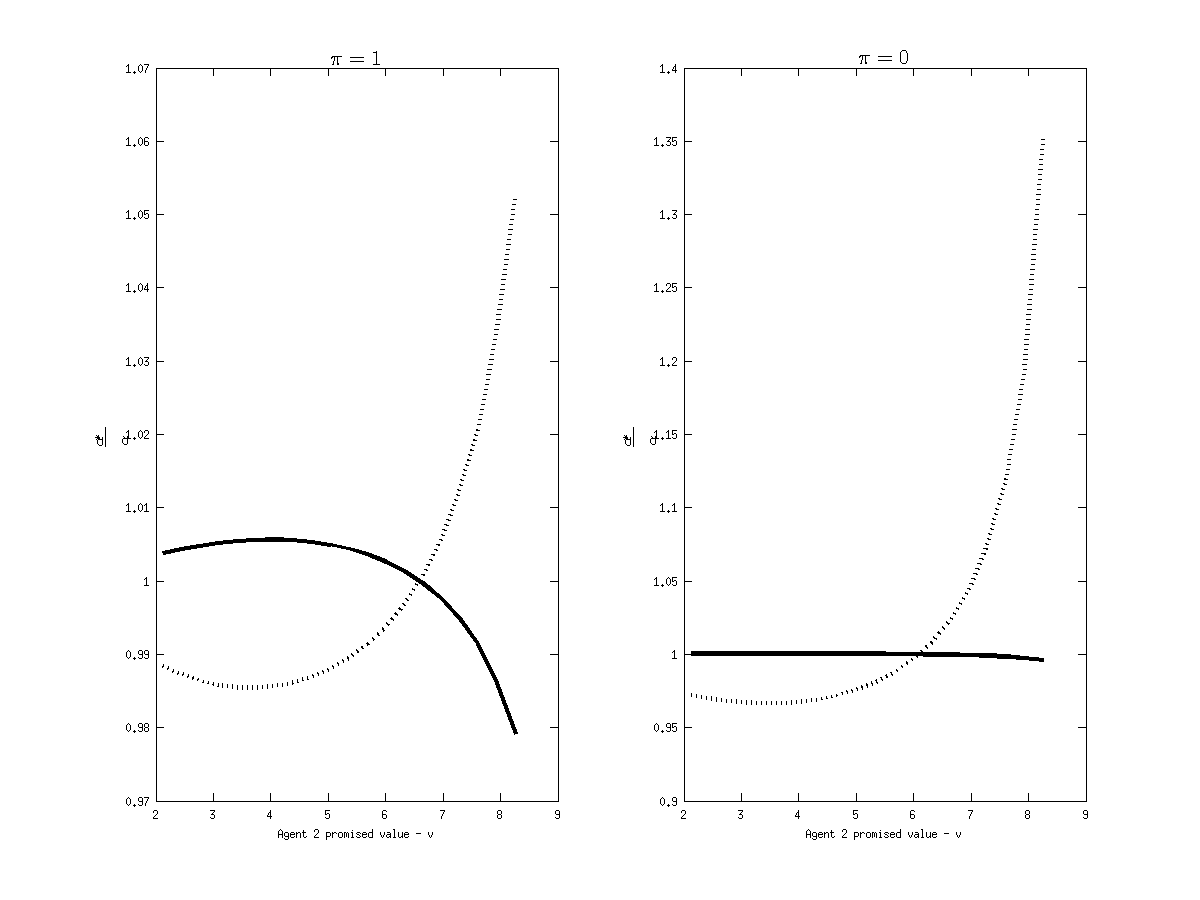
\includegraphics[scale=0.4]{Matlab/InfiniteHorizon/Learning/Plots/theta_1_finite/Transitory/AlphaStarNoLearning.png}

	\caption{This figure plots the gross change in consumption shares as a function 
of the initial promised value to Agent 2 given $y(z)=y_l$. The solid (dotted) line refers to
 $y(z^*)=y_l (y_h)$. The left (right) panel is the IID Model with $\pi=1$ ($\pi=0)$}
	\label{fig:AlphaStarNoLearning}
\end{figure} 
\noindent Figure \ref{fig:AlphaStarLearning} shows the evolution of consumption shares with type (II) ambiguity and $\theta_1=\infty$. The  dotted lines now refer to the realizations of $z^*$ corresponding to $s(z^*)=s_h$. The fact that the solid lines and the dotted lines do not overlap correponds to effect described in proposition \ref{propo-5} \footnote{In this case we have $\beta_m$ different across models}. Staring  from the allocation that insures consumption across realizations of the - $s$ shock, the relative wealth differences will tilt the common Bayes prior $\pi$ towards the IID model (Non-IID) in case $y(z)=y_hy(z)=y_l)$ since  good times are perceived to temporary. This distortion inturn implies that the model averaged probabilties of $z^*,z^{**}$ where $y(z^*)=y(z^**)$ will diverge across agents. Since the former allocation is now not consistent with optimality the planner will tilt it in a way that is consistent with the beliefs. For example in the case with $y(z)=y_l$ as in left panel. As 
Agent 2 gets wealthier, he relatively assigns more weight to the Non-IID model. This inturn implies that conditioning on the low aggregate endowment state ($y(z^*)=y_l$), he ends up assigning a higher probability to the event that $s(z^*)=s_l$. This relflects in higher consumption share of Agent 2 in $s_l$ as compared to $s_h$ for $y(z)=y_l$. With $\theta_1 <\infty$ the effect is ambiguous as conditional on the fact that consumption varies across the $s$ shock, the model specific transitions are distorted. The ultimate (non linear) effect on the model averaged probabilities coming from distorted priors and distorted transistions cannot be disentagled and depends on $\theta_1$,$\theta_2$ amognst other paarameters.
\begin{figure}[htbp]
\centering
	  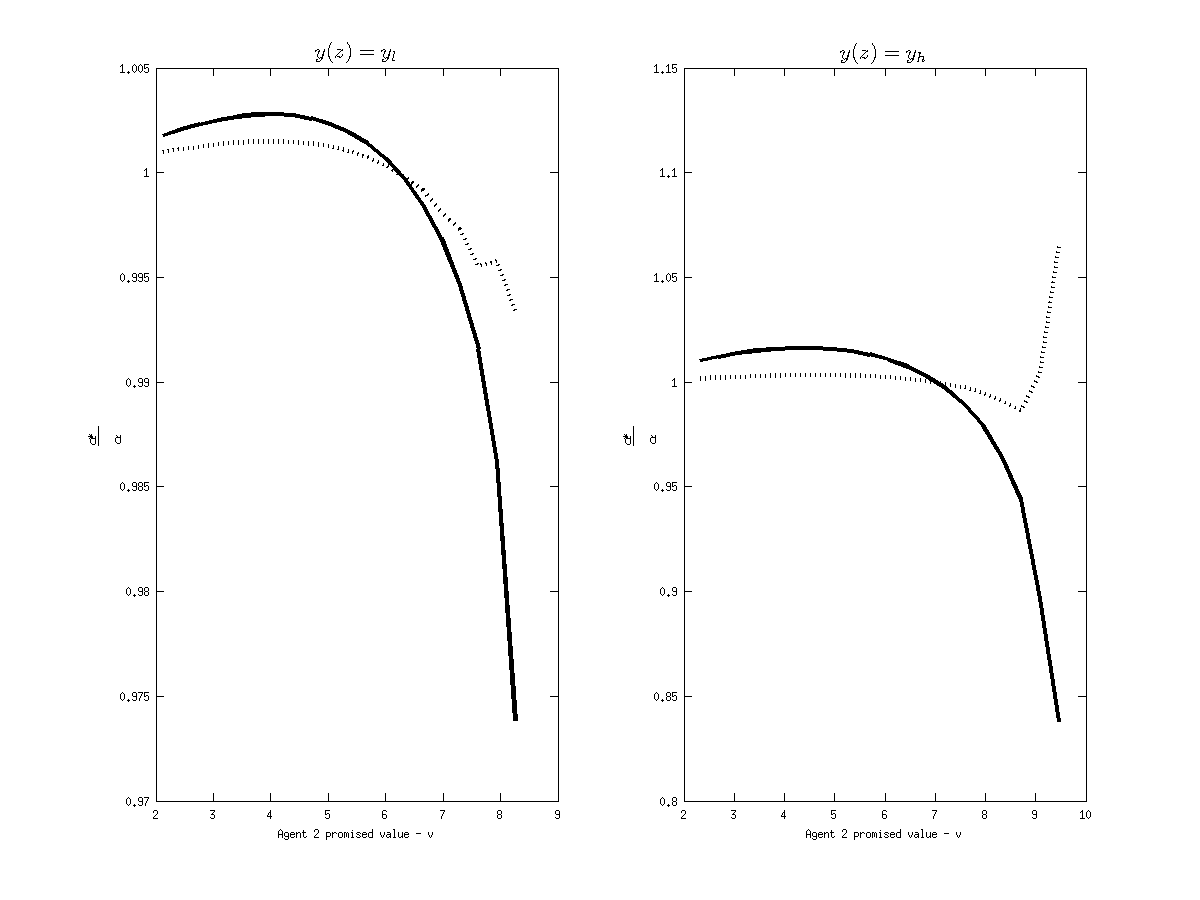
\includegraphics[scale=0.4]{Matlab/InfiniteHorizon/Learning/Plots/theta_1_infty/Transitory/AlphaStarLearning.png}

	\caption{ This figure plots the gross change in consumption shares as a function 
of the initial promised value to Agent 2 - v keeping $y(z^*)=y(z^{**})$ and $\pi=0.5$. The solid (dotted) line refers to
 $s(z^*)=s_l (s_h)$. The left (right) panel is the $y(z)=y_l(y_h)$}
	\label{fig:AlphaStarLearning}
\end{figure} 
%\noindent Figure \ref{fig:AlphaStarLearning} shows the evolution of consumption shares for type (II) ambiguity . The dotted lines now refer to the realizations of $z^*$ corresponding to $s(z^*)=s_h$. The fact that the solid lines and the dotted lines do not overlap correponds to effect described in proposition \ref{propo-5}. In this case the condition (2) is not satisfied. Consider a case when $\theta_1=\infty$ 
%and  $theta_2 <\infty $, 


\subsection{Distorted Beliefs}
The heterogeneity in agents due to the choice of initial promised value creates a differential wedge between the worst case beliefs of the agents and the underlying common approximating model. The magnitude of this wedge is captured by the relative entropy . We can compute the reltive entropy for the distribution of $P(z^{*}|z,m)$ and $\pi(m)$  indepedently. For brevity, Figure \ref{fig:EntropyMarginal} shows the the relative entropy of the marginal distribution of $z^{*}|z$ given $\pi$ since this is what matters for allocating consumption. Since we have $\gamma < 1$, the wealthier agent who bears most of the aggregate risk distorts most. This is reflected in \ref{fig:MarginalEntropy}. As $v \to v_{max}$ we see that the Agent 2's relative entropy is higher than Agent 1. 

{\[\mathcal{E}_{P,Q} =  \mathbb{E} \frac{\tilde{p}^i(z^*|z,\pi)}{p(z^*|z,\pi)} \log\left[\frac{\tilde{p}^i(z^*|z,\pi)}{p(z^*|z,\pi)}\right]\]}
\begin{figure}[htbp]
\centering
	  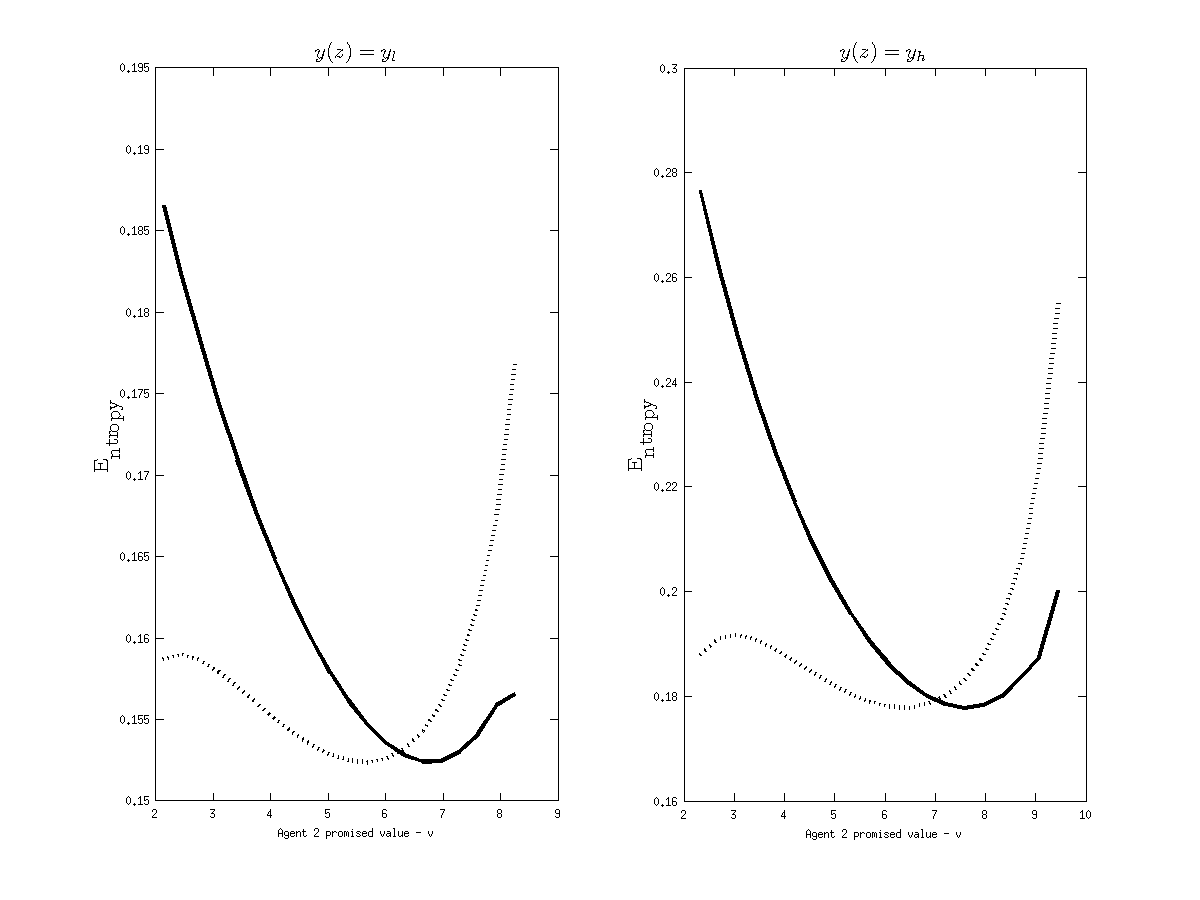
\includegraphics[scale=0.35]{Matlab/InfiniteHorizon/Learning/Plots/theta_1_finite/Transitory/EntropyMarginal.png}

	\caption{\small{This figure plots the relative entropy of the model averaged
 conditionals for both the agents. The solid (dotted) line refer to Agent 1 (Agent 2). The left (right) panel has $y(z)=y_l (y_h)$ and $\pi=0.5$ }}
 
	\label{fig:EntropyMarginal}
\end{figure} 

\noindent Figure \ref{fig:DistPriors} plots how the model priors diverge across agents. I plot the surface $\frac{\tilde{\pi}^2}{\tilde{pi}^1}[\pi,v]$ for $z=1$ and $z=3$ across the panelsfor the case with $\theta_1=\infty$.  As $v\to v^{max}$ this ratio is greater (less) than one if $y(z)=y_l$. This reflects the fact that wealthy agent (here Agent 2) relatively (to Agent 1) distrots the model prior $\pi$ in the direction of the Non IID model (making the ratio < 1) or the model with more persistence since he beleives bad times persist longer. A further observation is the apparent assymtery in $\pi$ and symmetery in $v$. The later comes from the fact that the agents are otherwise homogenous and $v$ ranging from $0$ to $v^{max}$ picks up all possible initial Pareto weights. The assymtery in $\pi$ is heuristically explained as follows:
\[\frac{\tilde{\pi} }{\pi} = \frac{1}{\pi+(1-\pi) \left(\frac{-V(\text{Non IID}) + V(\text{IID})}{\theta_2}\right)}\]
Notice that this ratio limits to $1$ when $\pi \to 1$ and to $\left(\frac{V(\text{Non IID}) - V(\text{IID})}{\theta_2}\right)$ as $\pi \to 0$. This is reflected as flattening out of the surface along the $\pi$ dimension in both the panels
\begin{figure}[htbp]
\centering
	  \includegraphics[scale=0.5]{Matlab/InfiniteHorizon/Learning/Plots/theta_1_infty/Transitory/DistortedPriors.png}

	\caption{This figure plots the $\frac{\tilde{\pi}^2}{\tilde{pi}^1}$ as a function of $v,\pi$. The left (right) panel has $y(z)=y_l (y_h)$ }
 
	\label{fig:DistPriors}
\end{figure} 


\subsection{Market Price of Risk}
\label{sec-MPR}
Figure \ref{fig:MarketPriceOfRiskNoLearning} plots the conditional market price of risk as a function of $v$. Note the U-shaped curve indicating higher market price of risk at extremes of wealth distributions. The solid (dotted) line reflects MPR in low aggregate endowment states and the dot-dashed lines are the values under the benchmark. Evidently market price of risk is higher than the benchmark but not countercylical in the Non IID model (right). With $\theta_2 < \infty$, the cylical properties depend on $\pi$. Figure \ref{fig:MPRLearningPi} depicts how presence of type (II) ambiguity affects cylical properties of market price of risk. The left panel plots MPR[$y_l$] (solid)and MPR[$y_h$] (dotted) for a choice of $v > \bar{v}$ as a function of $\pi$ with $\theta_2<\infty,\theta_1=\infty$. The right panel plots the same objects under the benchmark (with $\theta_1,\theta_2=\infty$ ). Since the first model is IID and the second model has persistence, the model averaged $\alpha\geq\frac{1}{2}$. Consistent 
with \ref{propo-6} the right panel has uniformly pro-cyclic market price of risk. However in the left panel we see that for $\pi$ greater than $.4$, the solid line crossed the dotted line and reflects countercylical MPR.
\begin{figure}[htbp]
\centering
	  \includegraphics[scale=0.4]{Matlab/InfiniteHorizon/Learning/Plots/theta_1_finite/Transitory/MarketPriceofRiskNoLearning.png}

	\caption{\small {This figure plots the MPR as a function of the initial promised
value to Agent 2- v. The  solid (dotted) line refers to $y(z)=y_l (y_h)$. The
left (right) panel has $\pi=1 (\pi=0)$}}
	\label{fig:MPRNoLearning}
\end{figure} 

\begin{figure}[htbp]
\centering
	  \includegraphics[scale=0.5]{Matlab/InfiniteHorizon/Learning/Plots/theta_1_infty/Transitory/MPRLearningPi.png}

	\caption{ This figure plots the conditional market price of risk as function of $\pi$. The solid (dotted) line is $y(z)=y_l (y_h)$. The left panel has $\theta_2<\infty,\theta_1=\infty $ and the right panel has both $\theta_1,\theta_2=\infty$}
 
	\label{fig:MPRLearningPi}
\end{figure} 


\section{Long-run dynamics}
With $\gamma<1$ the setup introduces interesting long-run dynamics for wealth distribution and assets prices.

\subsubsection{Continuation Values}
In the recursive planner's problem, an important choice variable is the menu of future continuation values. These continuation values capture history dependence inherent in planner's trade offs. As alluded earlier, current beliefs depend on future utility of the agent or actions of the planner. Since these beliefs matter for optimality, they constraint the choices of the Planner today. A similar force is present in a context of a Ramsey problem with forward looking constraints (For eg. Kydland and Prescott [1982]). A common outcome of these setups is history dependence in actions - captured in this case with the state variable - promised continuation utility. Also noting the relationship between the continuation value and the Lagrange multiplier, dynamics of continuation values correspond to time varying Pareto planner's weights. In the benchmark case, the dynamics of continuation values depend significantly on the initial choice of state variables. Lemma \ref{lemma-1} summarizes a ``separation'' phenomenon 
that characterizes how initial states matter. 

\noindent In a decentralized economy, time varying continuation values manifests itself as dynamics of wealth distribution. Appendix A links the wealth distribution to promised continuation values. In the benchmark case we have a stark prediction for the dynamics of wealth distribution - with complete markets and homothetic preferences, the wealth distribution is static. However with uncertainty and the ensuing heterogeneous beliefs, the wealth distribution changes over time. With lower bounds on utility we saw that the agent who has the most wealth bears most of the aggregate risk, this increases the wedge between his worst case distribution and the underlying true measure. He also over-insures himself in the low aggregate endowment states. What this means is that he transfers more money to the poor agent in good times for transfers in the bad times. Consequently a series of good shocks drains his wealth and makes him poor. In terms of continuation utilities , they should adjust downward. This creates an 
equalizing force and the continuation utilities can be expected tp cluster around $\bar{v}(z)$ \footnote{With type (I) ambiguity,IID approximating model and $\gamma <1$, Anderson (2005) shows that Pareto weights stabilize around \emph{regular steady states} which would correspond to $\bar{v}(z)$ in my setup}. However with type(II) ambiguity the distributional shock $s^*$ also rellocates wealth and the resulting ergodic distribution depends crucially on whether $P_M$ has absorbing states or not. In numerical simulations discussed later it turns out that the ergodic distribution of $\lambda$ is not necessarily degenarte around 1 in these cases. The implication of this finding is that with type(II) ambiguity and wealth allocation through the distributional shocks can generate non - trivial long run wealth distributions. 


\noindent \ref{fig:LambdaStarLStarNoLearning} depicts the gross change in $\lambda$ against the initial promised value of Agent 2 for type(I) ambiguity.  As discussed we see that when v is low (Agent 2 is poor), $\frac{\lambda[z^*|z,\pi,v]}{\lambda} > 1$ for $z^* : y(z^*)=y_h$. The rise in the Pareto weights correspond to wealth transfers to the Agent 2. Since $\lambda$ and $v$ are linked by the Envelope theorem, changes is $\lambda$ are in some way `implemented'' by changes in the choice variable $v$.
\begin{figure}[htbp]
\centering
	  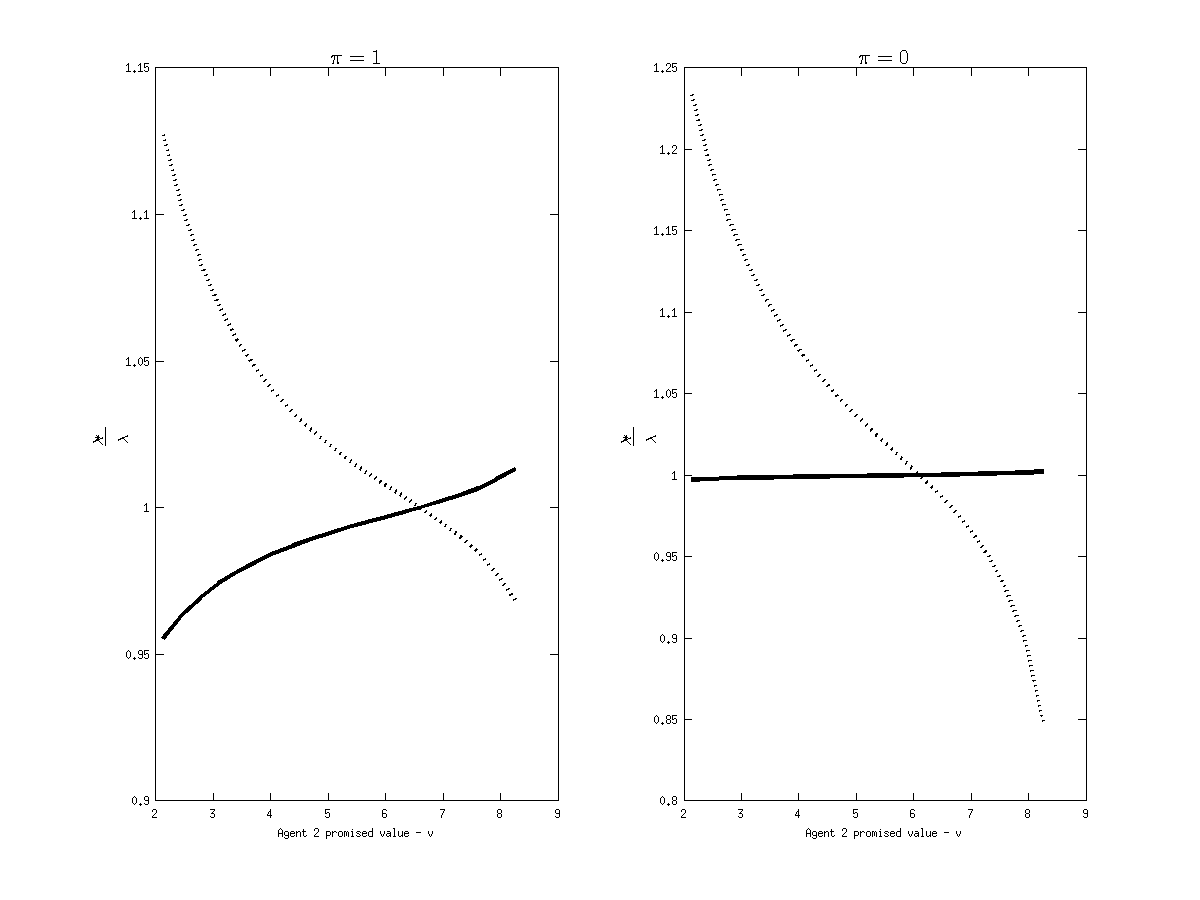
\includegraphics[scale=0.4]{Matlab/InfiniteHorizon/Learning/Plots/theta_1_finite/Transitory/LambdaStarLNoLearning.png}

	\caption{This figure plots the gross change in implicit Pareto weights as a function 
of the initial promised value to Agent 2 given $y(z)=y_l$. The solid (dotted) line refers to
 $y(z^*)=y_l (y_h)$. The left (right) panel is the IID Model with $\pi=1$ ($\pi=0)$}
	\label{fig:LambdaStarLStarNoLearning}
\end{figure} 


\begin{lemma}
Given $P_M$, $P_Z$ the stationary distribution of $z,\pi$ is given by $\Gamma^{SS}_z $ defined as a fixed point of the following functional equiation
\begin{equation}
\Gamma^{*}_{z^{*}}[\tilde {\pi}] =\int_{\pi}\sum_{z} \mathbb{I}_{\pi^*(z^*|z,\pi) \Gamma_z(d \pi)}
\end{equation}
Where $\Gamma_z(\tilde{\pi})= \text{Prob}\{z,\pi \leq \tilde{\pi}\}$ and $\pi^*$ is computed using Bayes rule
\end{lemma}

\begin{remark}
With $P_M=\mathbb{I}$, $\pi|m_0$ converges to $\delta_{m_0}(m)$ where $m_0$ is the first draw of $m_t$. In other cases with no absorbing cases, the ergodic distribution of $\pi$ has a non trivial support over a subset of $[0 \quad 1]$ in the case if two models. See Figure \ref{fig:PiBayesSS} for the ergodic distribution of $\pi$ with $P_M$ such that the models switch with a symmetric probability of $\frac{1}{10}$
\end{remark}


\begin{remark}
For $\theta_1,\theta_2=\infty$ we have the dynamics for $v^*$ given by 
\[ v(z^*|v,z,\pi)=\frac{v}{v^{max}[z,\pi]} v^{max}[z^*,\pi^*\]
\end{remark}

\begin{remark} 
For $\theta_1,\theta_2 <\infty$, there are two steady state distribution of continuation values.
\begin{enumerate}
	\item $v^max(z,\pi]$
	\item $\bar{v}(z,\pi)$
\end{enumerate}
 and $z,\pi$ follow $\Gamma^{SS}_z(\pi)$. For $\theta=\infty$ there are continuum of steady state distributions indexed by $\alpha$ 
 
\[V^{SS}_{\infty}(\alpha) \equiv \alpha v^{max}(z,\pi)\]
Where $(z,\pi)$ are distributed with $\Gamma^{SS}_z(\pi)$ as before and $\alpha \in [0 \quad 1]$
\end{remark}


In the figures below I discuss the ergodic distribution of $v^*$ for three cases when $\gamma <1$
\begin{enumerate}	
\item No Learning : $P_M=\mathbb{I}, \pi \in \{0,1\}$ 
The ergodic distribution takes two values for the (each corresponding to the realization of the aggregate endowment). Figures \ref{fig:SS_theta_1_finite_transitory} shows how the chain for $v^*$ clusters around the steady state distribution and that of $\lambda$ around 1.

\item Transitory Learning : $P_M=\mathbb{I},  \pi \in(0 \quad 1)$. 
The asymptotic dynamics of this are unchanged as $\pi^*$ converges to either 1 or 0 under Bayes rule. Learning here only contributes transient dynamics of quantities. The speed of learning is dictated by Bayes rule and in general depends on how ``different'' the models are.  A special cases that is particualry interesting is when $\theta_1=\infty$ and $\theta_2 < \infty$. The dynamics of wealth are driven by the ``survival'' mechanism discussed above untill learning is active and eventually the wealth distribution achieves a absorbing state. Starting from an inequal distribution the rich agent looses wealth on average till the ambiguity about the data generating model is active. If learning is ``slow'' the other agent has time to catch up. Figure \ref{fig:SS_theta_1_infty_transitory} shows the asymptotics of $v^*,\lambda^*$ in this case.

\item Persistent Learning : $P_M = [.9 .1;.1 .9]$
In this case the effects of learning persist in the limit. The steady state distribution of $\pi$ is shown in figure  \ref{fig:PiBayesSS} and has support over an interval of non-trivial length. This smooths out the ergodic distribution and is depicted in figures \ref{fig:SS_theta_1_finite_persistent} and \ref{fig:SS_theta_1_infty_persistent}
\end{enumerate}

\begin{figure}[htbp]
\centering
\subfloat[Dynamics for $v$]{
	  \includegraphics[scale=0.4]{Matlab/InfiniteHorizon/Learning/Plots/theta_1_finite/Transitory/VSS.png}
	}
	\subfloat [Dynaics for $\lambda$]{

	  \includegraphics[scale=0.4]{Matlab/InfiniteHorizon/Learning/Plots/theta_1_finite/Transitory/LambdaSS.png}
}
\caption{\small {This figure plots the ergodic distribution for $v^*$,$\lambda^*$ with $\theta_1=.5,\theta_2 =.5$ and $P_M=\mathbb{I}$}}
\label{fig:SS_theta_1_finite_transitory}
\end{figure} 

\begin{figure}[htbp]
\centering
\subfloat[Dynamics for $v$]{
	  \includegraphics[scale=0.4]{Matlab/InfiniteHorizon/Learning/Plots/theta_1_infty/Transitory/VSS.png}
	}
	\subfloat [Dynaics for $\lambda$]{

	  \includegraphics[scale=0.4]{Matlab/InfiniteHorizon/Learning/Plots/theta_1_infty/Transitory/LambdaSS.png}
}
\caption{\small {This figure plots the ergodic distribution for $v^*$,$\lambda^*$ with $\theta_1=\infty,\theta_2 =.5$ and $P_M=\mathbb{I}$}}
\label{fig:SS_theta_1_infty_transitory}
\end{figure} 



\begin{figure}[htbp]
\centering
\subfloat[Dynamics for $v$]{
	  \includegraphics[scale=0.4]{Matlab/InfiniteHorizon/Learning/Plots/theta_1_finite/Persistent/VSS.png}
	}
	\subfloat [Dynaics for $\lambda$]{

	  \includegraphics[scale=0.4]{Matlab/InfiniteHorizon/Learning/Plots/theta_1_finite/Persistent/LambdaSS.png}
}
\caption{\small {This figure plots the ergodic distribution for $v^*$,$\lambda^*$ with $\theta_1=.5,\theta_2 =.5$ and $P_M\neq \mathbb{I}$}}
\label{fig:SS_theta_1_finite_persistent}
\end{figure} 



\begin{figure}[htbp]
\centering
\subfloat[Dynamics for $v$]{
	  \includegraphics[scale=0.4]{Matlab/InfiniteHorizon/Learning/Plots/theta_1_infty/Persistent/VSS.png}
	}
	\subfloat [Dynaics for $\lambda$]{

	  \includegraphics[scale=0.4]{Matlab/InfiniteHorizon/Learning/Plots/theta_1_infty/Persistent/LambdaSS.png}
}
\caption{\small {This figure plots the ergodic distribution for $v^*$,$\lambda^*$ with $\theta_1=\infty,\theta_2 =.5$ and $P_M\neq \mathbb{I}$}}
\label{fig:SS_theta_1_infty_persistent}
\end{figure} 



Note that in \ref{fig:SS_theta_1_finite_persistent}, \ref{fig:fig:SS_theta_1_infty_persistent} the chain for $\lambda$  does not cluster around at $1$.


\subsection{Dynamics of Market Price of Risk}

%XXXX WHEN IS MARKET PRICE OF RISK COUNTERCYLICAL. REWORD THIS SECTION AFTER YOU FIGURE OUT MORE DETAILS ABOUT CYLICITY OF MPR
%
%
As discussed in section \ref{sec-Pricing Kernel}  and \ref{sec-MPR} the conditional market price of risk depends on the state - $(z,\pi,v)$. The dynamics of $v$ thus feed into the dynamics of market price of risk . As long as $\pi$ is not degenerate, the market price of risk displays volatility conditioned on the aggregate shocks.  
%
%Even in the Benchmark Model presence of hidden state by itself adds some time-variation in market price of risk since posteriors converge to the steady state distribution. Is this time-variation also state dependent ? Note that the symmetry in the way the transition matrices are constructed under each model makes market price of risk acyclic. With $\theta_1,\theta_2 = \infty$, we have
%\[MPR_t \approx \gamma \sigma_t(\Delta y_{t+1})\]
%Under both models the change is $(\Delta y_{t+1})^2$ is independent of the the current state.  
%\footnote{In an Linear Gaussian setup this is naturally true since the posterior variances are independent of signal realizations} However, with ambiguity the agents additionally tilts the outcome of learning towards the Non-IID model in low endowment states and vice versa. This leads to countercyclical market price of risk.
%
In the figures below I simulate a path for the market price of risk from the same stationary distributions as in the previous sections. Figure \ref{fig:MPRDraw_theta_1_finite_transitory} depict the dynamics of MPR for type (I) ambiguity. With the IID model we have the MPR is flat (but higher than what it would have been with $\theta_1=\infty$). The Non-IID transient model has the block like structure where MPR is constant across realizations of the distributive shock -$s^*$. Finally figure \ref{fig:MPRDraw_theta_1_finite_persistent} and \ref{fig:MPRDraw_persistent} depict dynamics when $P_M\neq \mathbb{I}$ and type (II) ambiguity is active asymptotically. The MPR now moves around within periods of low (high) realizations of aggregate endowment.
\begin{figure}[htbp]
\centering
	  \includegraphics[scale=0.4]{Matlab/InfiniteHorizon/Learning/Plots/theta_1_finite/Transitory/MPRDraw.png}

	\caption{\small {This figure plots a sample path of MPR from the ergodic distribution for $\theta_1,\theta_2 =.5$ and $P_M=\mathbb{I}$}. The shaded bars have $y(z)=y_l$}

	\label{fig:MPRDraw_theta_1_finite_transitory}
\end{figure} 

\begin{figure}[htbp]
\centering
\subfloat[MPR $\theta_1<\infty,\theta_2<\infty$]{
	  \includegraphics[scale=0.4]{Matlab/InfiniteHorizon/Learning/Plots/theta_1_finite/Persistent/MPRDraw.png}
	}
	\subfloat [MPR $\theta_1=\infty,\theta_2<\infty$]{

	  \includegraphics[scale=0.4]{Matlab/InfiniteHorizon/Learning/Plots/theta_1_infty/Persistent/MPRDraw.png}
}
%\caption{\small {This figure plots the ergodic distribution for $v^*$,$\lambda^*$ with $\theta_1=\infty,\theta_2 =.5$ and $P_M\neq \mathbb{I}$}}
\label{fig:MPRDdraw_persistent}
\end{figure} 

%\begin{figure}[htbp]
%\centering
%	  \includegraphics[scale=0.4]{Matlab/InfiniteHorizon/Learning/Plots/Fig_MPR1.png}
%
%	\caption{This figure plots the Market Price of Risk for sample of 150 periods from the
%          ergodic  distribution.. The shaded bars are periods of low aggregate endowment}
%	\label{fig:MPRPL}
%\end{figure} 
%
%
%\begin{figure}[htbp]
%\centering
%	  \includegraphics[scale=0.4]{Matlab/InfiniteHorizon/Learning/Plots/Fig_MPR2.png}
%
%	\caption{This figure plots the Market Price of Risk for sample of 150 periods from the
%          ergodic  distribution.. The shaded bars are periods of low aggregate endowment}
%	\label{fig:MPRPL}
%\end{figure} 
%
%\begin{figure}[htbp]
%\centering
%	  \includegraphics[scale=0.4]{Matlab/InfiniteHorizon/Learning/Persistent/Plots/Fig_MPR1.png}
%
%	\caption{This figure plots the Market Price of Risk for sample of 150 periods from the
%          ergodic  distribution.. The shaded bars are periods of low aggregate endowment}
%	\label{fig:MPRPL}
%\end{figure} 

\section{Review - Complete Markets}

\section{Incomplete Markets}
In the previous sections we saw how wealth driven relative disgreements affected insurance choices in presence of complete markets. The distributional shock played a role similiar to a sun spot variable or a betting device where by agents could trade on differences in beliefs. The source of this differences came from the fact that poorer agents held held relatively a smaller proportion of aggregate risk and hence resolved the uncertainty about the underlying model (IID or Persistent) differently. Infact in absence of aggregate risk these mechanism do not have a bite in complete markets \footnote{Refer Proposition \ref{propo-2}}. With uninsurable idiosyncratic risk wealth differences matter inspite of no aggregate risk. To study this I will consider two settings without aggregate risk differing in why there is uninsurable risk. 

In the first setup market incompleteness is exogenous - There is only a riskless bond that can be traded. The supply of this bond is exogenous. The source of heterogenity in this economy is share of initial bond holdings. The key mechanism here is that with sufficient assets the agents can \emph{self insure} themselves. Thus relative pessimism and differences in beleifs about the data generating model depends relative differences in the initial asset holdings.

For the second setting , market incompleteness is driven by private information. In a simple example, I solve a second-best version of Planner's problem with allocations satisfying both a promise-keeping and incentive constraints. The tension in this setting is that optimal insurance requires tilting the consumption shares in favor of the agent who perceives the contingency more likely, but incentive constraints restrict the shape of the contract. I will contrast the resulting contract with a appropiate benchmark isolating the concerns from ambiguity. 


\section{Bond Economy}
This section describes a bond economy without aggregate risk. The agents are identical with respect to the their endowment shocks and differ in the initial asset holdings. I first begin with a static (partial equilibrium) example explaining how the resolution of model uncertainty depends on the asset levels. Particulary note that $\gamma$ plays a minimal role here in driving the results.

\subsection{Static case}
Consider an agent with a risky endowment $y$. The support for $y$ is such that consumption is non-ngeative even for the worst income shock. The agent has risk free assets which pays $b$. 
\[c(y,b)=y+b\]

\[V^R (b)=\min_{m}\mathbb{E}m[u(c)+\theta\log(m)]\]
such that 
$Em=1$
 
\begin{proposition}
\label{propo-9}
For every $b$ there exists a threshold $\bar{y}(b)$ such that $\frac{\partial m(y,b)}{\partial b} >0 \text{iff} y>\bar{y}(b)$
\end{proposition}
\begin{proof}
The choice for $m^*$
\[m^*(y,b)\propto \exp\left\{\frac {-(y+b)^{1-\gamma}}{\theta(1-\gamma)}\right\}\]
taking logs and differentiating with respect to $b$ we have
\[\frac{\partial \log{m^*(y,b)}}{\partial b} = -\frac{(y+b)^{-\gamma}}{\theta}  + \frac{\mathbb{E} \exp \left\{ -\frac{(y+b)^{1-\gamma}}{(1-\gamma)\theta}\right\} (y+b)^{-\gamma}} {\theta \mathbb{E} \exp \left\{ -\frac{(y+b)^{1-\gamma}}{(1-\gamma)\theta} \right\}}\]
Define $\tilde{p}(y)=p(y)\frac{ \exp \left\{ -\frac{(y+b)^{1-\gamma}}{(1-\gamma)\theta}\right\} } { \mathbb{E} \exp \left\{ -\frac{(y+b)^{1-\gamma}}{(1-\gamma)\theta} \right\}}$
we have
\[\frac{\partial d \log{m^*(y,b)}}{\partial b} = -\frac{(y+b)^{-\gamma} - \tilde{\mathbb{E}}(y+b)^{-\gamma}}{\theta}\]
Let $\bar{y}(b)$ be such that the numerator is zero
\[\bar{y}(b) = \left(\tilde{\mathbb{E}} (y+b)^{-\gamma}\right)^{-\frac{1}{\gamma}}-b\]
Since $y+b\geq 0$ as $y>\bar{y}(b)$ we have 
\[\frac{\partial d \log{m^*(y,b)}}{\partial b}>0\]
\end{proof}
Since $\tilde{p}(y)=p(y)m^*(y,b)$ we have that the richer the agent overweights  ``sufficiently'' good realizations of $y$. The intuation is that with higher $b$ the realtive fluctations in $y$ are not large enough to distort the distribution of $y$. Large assets provide the buffer for self-insurance and hence reduce concerns for model uncertainty. 

Figure \ref{fig:StaticBondEconomy} shows an example with $\theta=1$ and $\gamma=.5$ and a risky endowment $y$ that has a density propotional to a standard normal. The solid line depicts the density under the approximating model. The two dotted lines show how the worst case density ``shifts'' we change the asset levels. In particular the dotted red line being closer to the benchmark illustrates the self-insurance effect of high assets. Figure \ref{fig:StaticYBar} shows how the threshold $\bar{y}(b)$ flattens out as $b$ increases. The shaded region are the realizations of $y$ that are relatively overweigted by the marginally `rich' agent.
	\begin{figure}[htbp]
\centering
	  \includegraphics[scale=0.5]{Matlab/IncompleteMarkets/Plots/StaticBondEconomy.png}

	\caption{This figure shows the reference and worst case models for two levels of assets in the static example with $\theta=1$,$\gamma=0.5$}
	\label{fig:StaticBondEconomy}
\end{figure} 

	\begin{figure}[htbp]
\centering
	  \includegraphics[scale=0.5]{Matlab/IncompleteMarkets/Plots/StaticYBar.png}

	\caption{This figure plots $\bar{y} (b)$ for the static example with $\theta=1$,$\gamma=0.5$. The shaded region are realizations of $y$ for which $m^*_b(y,b)>0$}
	\label{fig:StaticYBar}
\end{figure} 

%
%In the next section I will study this mechanism in a simple 2 period equilibrium model. 
%\subsection{Setup}
%This settings modifies the complete market setting to restric the set of assets to risk-free bond. The preferences and technology are same as the complete market setting. I first study the case with no aggregate risk or $y_l=y_h=y$. Denote the initial assets of Agent 1 by $b_{0,1}$. 
%
%\subsection{Equilibrium}
%Given $z,\pi,b$ and $q$- price of the bond each agent solves for optimal consumption and bond holdings by maximizing
%\begin{equation}
%Q(b,z,\pi)=\max_{c,b^*}{\mathbb{T}^2_{\theta,2}\left[u(c)+\delta\mathbb{T}^{1}_{\theta,m}Q^{*}(b^*,z^*,\pi^*)\right]}
%\label{eq:HHProblemBond}
%\end{equation}
%subject to
%\[c+qb^*=y(z)s(z)+b\]
%
%With two periods we have $Q^*(b^*,z^*,\pi^*)=u[y(z^*)s(z^*)+b^*]$. Using this we can solve for the consumption-savings decision
%\[\mathcal{B}(b,z,\pi,q) : q u_{c}[y(z)s(z)+b-qb^*]-\delta\tilde{\mathbb{E}}Q_{b}^{*}(b^*,z^*,\pi^*)=0\]
%The market clearing $q$ solves the following fixed point for a given choice of $(b_{0,1},z,\pi)$
%\begin{equation}
%\mathcal{B}(b_{0,1},z,\pi,q)+\mathcal{B}(-b_{0,1},z,\pi,q)=0
%\label{eq:BondPrice}
%\end{equation}
%
%%\begin{figure}[htbp]
%%\centering
%%	  \includegraphics[scale=0.4]{Matlab/IncompleteMarkets/Plots/Fig_AssetDemands_0.png}
%%
%%	\caption{This figure plots the asset demands for both the agents in
%%          both income states for the IID  Model. The  solid lines are
%%          aggregates and the blue(red) dotted line refers to Agent 1
%%          (Agent 2)}
%%	\label{fig:bstar}
%%\end{figure}
%\subsection{Analysis}
%As long as we have $ys_l< \bar{y}[\mathcal{B}(b_{0,1},z,\pi,q)]<ys_h$ \footnote{A sufficient condition is $b_{0,1} \geq \underbar{b}_{0,1}$ and $\bar{y}'(b) >0$},Propostion \ref{propo-9} implies a negative association of assets levels and pessimism. Define ``relative pessimism'' as the worst case ratio of probabilities of low income shock tomorrow. 
%\[\mathcal{R}(z,\pi,b_{0,1})=\frac{\tilde{Pr}^{1}[s(z^*)=s_{l}]}{\tilde{Pr}^{2}[s(z^*)=s_{h}]}\]
%
%The following graphs \ref{fig:BondEconomyOucomes} and \ref{fig:BondEconomyBeleifs} plot the outcomes (consumption,savings,bond prices) and the belief disagreements for an example with $\theta_1=\theta_2=1,\gamma=\frac{1}{2}$. The dotted lines represent the benchmark with $\theta_1,\theta_2=\infty$. In figure \ref{fig:BondEconomyOucomes}  we see that savings of Agent 1$b^*=\mathcal{B}$ approches $-ys_l$ and consumption goes to 0 as $b_{0,1}$ approches $\underbar{b}_{0,1}$. We see that $q$ is higher than the benchmark as ceterus paribas, model uncertainty accenutuates the precautionary motive. Notice that at $b_{0,1}$ near $\underbar{b}_{0,1}$ Agent 1 borrows more than the benchmark. The last plot in the bottom panel plots $\bar{y}[\mathcal{B}[(b_{0,1}]$. As proposition \ref{propo-10} predicts, $\bar{y}$ approaches $ys_l$ from the right and the fact that it lies between $ys_l$ and $ys_h$ for all intermediate $b_{0,1}$ satisfies the conditions of Proposition \ref{propo-9}. Figure \ref{fig:BondEconomyBeleifs} (
top panel) now shows the ``relative pessimism'' $\mathcal{R}$ as defined above. We see that it dimishes with $b_{0,1}$. The bottom pael shows the distorted model priors for both the agent.  With $b_{0,1}$ low , Agent 1 (solid line) tilts the prior ($\pi=0.5$) towards the persistent model when he receives the low income shock. This twisting is moderated and $\tilde{\pi}$ goes towards $\pi$ as $b_{0,1}$ becomes large. The opposite holds for Agent 2
%	\begin{figure}[htbp]
%\centering
%	  \includegraphics[scale=0.5]{Matlab/IncompleteMarkets/Plots/BondEconomyOucomes.png}
%
%	\caption{The top panel plots the bond price , Agent 1's bond demand as a function of his initial bond holdings $b_{0,1}$. The dotted line are the outcomes in the benchmark case without ambiguity. The bottom panel plots Agent 1's consumption and $\bar{y}(b^*_1)$ respectively. In all the plots $z=1$ and $\pi=.5$}
%	\label{fig:BondEconomyOucomes}
%\end{figure} 
%	\begin{figure}[htbp]
%\centering
%	  \includegraphics[scale=0.5]{Matlab/IncompleteMarkets/Plots/BondEconomyBeleifs.png}
%
%	\caption{The top panel plots the relative pessimism as a function of Agent 1's share of initial assets-$b_{0,1}$. The bottom panel plots $\tilde{\pi}$ for both the agents with the solid line depicting Agent 1. In all the plots $z=1$ and $\pi=.5$ }
%	\label{fig:BondEconomyBeleifs}
%\end{figure} 
%
\section{Bond Economy}
This section describes the bond economy version of the earlier setup without aggregate risk  : $y_s=y_l=\bar{y}$ and normalizing aggregate supply of bonds to zero. We further compress the state $z$ and the transition matrix $P_Z(z^*|z,m)$ to $P_S(s^*|s,m)$ . For the nuemrical analysis. I impose symmetry on  $P_S(s^*|s,m)$ to obtain a parsimonius paraterization (with $\alpha^{S}(m)$ ) as follows
\[P_S(s^*|s,m)=\bordermatrix{~ & s_l & s_h \cr
														s_l & \alpha^S(m) & 1-\alpha^S(m) \cr
														s_h & 1-\alpha^S(m) & \alpha^S(m) \cr} \]

\noindent The endowments of Agent 1 and Agent 2 are $ys$, $y(1-s)$ respectively. Note that $s$ is not an \emph{idiosyncratic} shock as all agents of type 1 have the same endowment. This allows us to aggregate symmetric decisions over individual types of agent and keep track only of how weatlh is ditributed across types. With the zero aggregate supply of bonds and common initial priors - $\pi_0$, the sufficient state variables for this economy are $(B^1, s, \pi)$   :- The assets of Agent 1, current realization of the distributional shock and the Bayes prior on the unobservable state - $m$.

\subsection{Agents problem}
\noindent Given bond prices $q$, let $Q^i(b,B^1,s,\pi)$ be the value of Agent i with assets b and aggregate state $(B^1,s,\pi)$

\begin{equation}
\label{BEAgent1ValueFunction}
\mathcal{Q}^1(b,B^1,s,\pi)=\max_{c,b^*} { \mathbb{T}^2_{\theta_2} \left[u(c)+\delta \mathbb{T}^1_{\theta_1,m}\mathcal{Q}^1 (b^*,B^{1*},s^*,\pi^*)\right]}
\end{equation}
subject to
\begin{subequations}
\begin{equation}
c+qb^*=ys+b
\end{equation}
\begin{equation}
\pi^* \propto \sum_{m}{P_M(m^*|m)P_S(s^*|s,m)\pi(m)}
\end{equation}
\begin{equation}
b^* \geq \underbar{b}^1(s)
\end{equation}
\end{subequations}

Where $\underbar{b}^1(s)$ is the natural debt limit for Agent 1 in state $s$

Similiarly we can describe Agent 2's problem as  
\begin{equation}
\label{BEAgent2ValueFunction}
\mathcal{Q}^2(b,B^1,s,\pi)=\max_{c,b^*} { \mathbb{T}^2_{\theta_2} \left[u(c)+\delta \mathbb{T}^1_{\theta_1,m}\mathcal{Q}^2 (b,B^{1*},s^*,\pi^*)\right]}
\end{equation}
subject to
\begin{subequations}
\begin{equation}
c+qb^*=y(1-s)+b
\end{equation}
\begin{equation}
\pi^* \propto \sum_{m}{P_M(m^*|m)P_S(s^*|s,m)\pi(m)}
\end{equation}
\begin{equation}
b^* \geq \underbar{b}_2 (s)
\end{equation}
\end{subequations}
Where $\underbar{b}^2(s)$ is the natural debt limit for Agent 2 in state $s$. 
\begin{remark}
Along equilibrium paths market clearing will impose upper limits on asset postions of individual agents too
\end{remark}
%
Given $q$, the interior solutions to these problems pin down the consumption savings decisions of both agents. Let
 $\mathcal{B}^i[b,B^1,\pi,s,q]$ be the savings of Agent i.
 
 \begin{subequations} 
 \label{SavingsPolicy}
 \begin{equation}
\mathcal{B}^1(b,B^1,s,\pi,q) : q u_{c}[ys+b-qb^*]-\delta\tilde{\mathbb{E}}^1_{s}Q^1_{b}(b^*,B^{1*},s^*,\pi^*)=0
\end{equation}
\begin{equation}
\mathcal{B}^2(b,B^1,s,\pi,q) : q u_{c}[y(1-s)+b-qb^*]-\delta\tilde{\mathbb{E}}^2_{s}Q^2_{b}(b^*,B^{1*},s^*,\pi^*)=0
\end{equation}
\end{subequations}
The expectations are taken with respect to the worst case -model-averaged marginals $\sum_{m}\tilde{\pi}^i(m)\tilde{P}^i_S(s^*|s,m)$. Like before $\tilde{\pi}^{i}$ and $\tilde{P}^i_S$ can be computed using the value functions $Q^i$ for each agent.
%
%
%
\subsection{Recursive Competitive Equilibrium}
Given $(B^{1}_{-1,0}, s_0, \pi_0)$ a recursive comptetitive equilibrium is set of value function,policy rules for each agent - $\{\mathcal{Q}^i,\mathcal{B}^i\}_{i=1,2}$ and bond prices $q$ such that given $q$, the value functions and policy rules solve the agents problems and bonds markets clear
\[q(B^1,s,\pi) : \mathcal{B}^1(B^1,B^1,s,\pi,q)+  \mathcal{B}^2(-B^1,B^1,s,\pi,q)=0\]
\subsection{Bond Economy : A Minimally Stochastic case}
I first analyze the equilibrium under special dynamics for $s$ which reduces the problem essentially to a 2 period version that can be quickly solved and study how wealth differences affect the worst case beliefs of agents. This deactivates the effects of distorted filtering and long run dynamics which are taken care in the next section. 
The simple economy is constructed under the following dynamics for $\{s_t\}_{t>0}$ given $s_0$
\begin{enumerate}
	\item $s_1|s_0 \sim P_S[s^*|s,m]$
	\item $s_{t+1}=s_{t}$ for $t\geq1$ 
\end{enumerate}
This is a \emph{minimally stochastic case} which features an absorbing state for $s_t$ from $t=1$. 
The value of the agent can now be computed backwards -  Let $\mathcal{Q}^{i *}$ be the value of Agent i from period 1 onwards and $\mathcal{Q}^{i 0}$ denote the value after $s_0$ has been realized. The stationary environment after period 1 implies that 
\begin{itemize}
	\item $\mathcal{Q}^{1*}[b,B^1,s,\pi]=\frac{u[ys+(1-\delta)b]}{1-\delta}$ and $\mathcal{B}^{1*}[b,B^1,s,\pi]=b$
	\item $\mathcal{Q}^{2*}[b,B^1,s,\pi]=\frac{u[y(1-s)+(1-\delta)b]}{1-\delta}$ and $\mathcal{B}^{2*}[b,B^1,s,\pi]=b$
	\item $q(B^1,s,\pi)=\delta$
\end{itemize}

Now we can derive the objects in $t=0$ using the above as terminal conditions. 
\begin{proposition}
\label{propo-10}
There exists a $\underbar{B}^1_{-1,0}[s,\pi]$ such that $\lim_{b\to \underbar{B}^1_{-1,0}} \mathcal{B}^{1,0}(b,\underbar{B}^1_{-1,0},s,\pi,q) = -\frac{ys_l}{1-\delta}$. Further we also have 
\[\lim_{b \to \underbar{B}^1_{-1,0}}\bar{y}[\mathcal{B}(b,\underbar{B}^1_{-1,0},s,\pi,q)] = ys_l\]
\end{proposition}
%
\begin{proof}
As $\mathcal{B}^{1,0}$ approches $-\frac{ys_l}{1-\delta}$, marginal utility of consumption of Agent 1 in $s^*=s_l$ diverges to $\infty$. For an interior solution, the FOC would require his current consumption to go to zero as well. This means that $\underbar{b}_{-1,0}[s,\pi]$ will satisfy
\[\underbar{b}_{0,1} \approx q \frac{ys_l}{1-\delta}-ys \]
and from Agent 2's FOC along with market clearing we have that $q$ is
\[q \approx \delta \frac{\tilde{\mathbb{E}}Q_b^{2*}(\frac{ys_l}{1-\delta},-\frac{ys_l}{1-\delta},s^*,\pi^*)}{u_c(y)}\]

This suggests $\underbar{b}_{-1,0}[s,\pi]=  \delta\left(  \frac{\tilde{\mathbb{E}}Q_b^{2*}(\frac{ys_l}{1-\delta},-\frac{ys_l}{1-\delta},s^*,\pi^*)}{u_c(y)}\right)\left(\frac{ys_l}{1-\delta}\right)-ys$

Following steps in \ref{propo -9}, the threshold for Agent 1's income to ensure that relative optmimism rises with assets satisfies 

\[\bar{y}[b^*]=\left(\check{\mathbb{E}}^{1}_{s} [ys^{*}+b^*(1-\delta)]^{-\gamma}\right)^{-\frac{1}{\gamma}} -(1-\delta)b^*\]

Note that the liklihood ratio $m(b^*,s^*)=\frac{\sum_{m} \tilde{\pi}^1(m)\tilde{P}^1_S(s^*|s,m)}{\sum_{m}{\pi(m)P_Z(s^*|s,m)}}$
The numerator can be simplified to
\[\left(\frac{\exp\{\frac{-u[ys^*+b^*(1-\delta)]}{\theta_1}\}}{\sum_{m} \exp\{\frac{-\delta \mathbb{T}^1_{\theta_1,m}[u(ys^*+b^*(1-\delta))]}{\theta_2}\}}\right)\sum_{m}{\pi(m)P_S(s^*|s,m) F^1(m)}\]
and $F^1(m)=\exp\left\{ \left( \frac{\theta_2-\delta \theta_1}{\theta_1\theta_2}\right)\mathbb{T}^1_{\theta_1,m}\  [u(ys^*+b^*(1-\delta))]\right\}$

The derivative  $\frac{\partial \log[m(b^*,s^*)]}{\partial b^*}$ is given by 

\[-\left( \frac{1-\delta}{\theta_1}\right) [ys^*+b^*(1-\delta)]^{-\gamma}+ (1-\delta) \sum_{m} \tilde{E}^1_{m,s}[ys^*+b^*(1-\delta)]^{-\gamma} \left( \frac{\delta}{\theta_2} \tilde{\pi}^1(m)+\left(-\frac{\delta}{\theta_2} +\frac{1}{\theta_1}\right) \hat{\pi}^{*}(m) \right) \]
where $\hat{\pi}^{*}(m) \propto \pi(m)P_S(s^*|s,m)F^1(m)$

Multipliying by $\frac{\theta_1}{1-\delta}$, we can define $\check{\pi}^{*}$ as $\frac{\delta \theta_1}{\theta_2}\tilde{\pi}^1+\left(1- \frac{\delta \theta_1}{\theta_2}\right)\hat{\pi}^*$.

Now $\frac{\partial \log[m(b^*,s^*)]}{\partial b^*} \geq 0$ if and only if $ys_h\geq \bar{y}[b^*]\geq ys_l$

\[\bar{y}[b^*]=\left(\check{\mathbb{E}}^{1}_{s} [ys^{*}+b^*(1-\delta)]^{-\gamma}\right)^{-\frac{1}{\gamma}} -(1-\delta)b^*\]


Now as $b\to \underbar{B}^1_{0,-1}[s,\pi]$ and $b^*=\mathcal{B}^{1,0}[b,s,\pi]\to -\frac{ys_l}{1-\delta}$
\[\bar{y}\left(\frac{-ys_l}{1-\delta},s^*\right)=ys_l\]
\end{proof}
As long as we have $ys_l< \bar{y}[\mathcal{B}(B^1,B^{1},s,\pi,q)]<ys_h$ \footnote{A sufficient condition is $B^{1} \geq \underbar{B}^{1}_{0,1}$} ,Propostion \ref{propo-9} implies a negative association of assets levels and pessimism. 
\subsection{Numerical Algorithm: General Case}

\begin{enumerate}
	\item Define a grid on $b,\pi$
	\item Guess some prices $q^k_{s}(b,\pi)$ and a non-negative function for the consumption policy rule $\mathcal{C}_{s}^{k(j)}(b,\pi)[i]$ where $s=s_l,s_h$
	\item Obtain the policy for savings using the budeget constraint 
	\[\mathcal{B}^{k(j)}_s(b,\pi)[1] = \frac{b+ys-\mathcal{C}^{k(j)}_{s}[b,\pi][1]}{q^k_{s}(b,\pi)}\]
	\[\mathcal{B}^{k(j)}_s(b,\pi)[2] = \frac{-b+ys-\mathcal{C}^{k(j)}_{s}[b,\pi][2]}{q^k_{s}(b,\pi)}\]
	\item Get an approximation for $Q^j[i]$ by iterating on 	\[Q^{k(j+1)}_{s}(b,\pi)[i]={\mathbb{T}^2_{\theta,2}\left[u(\mathcal{C}^{k(j)}_s[b,\pi][i])+\delta\mathbb{T}^{1}_{\theta,m}Q_{s^*}^{k(j)}(\mathcal{B}^{k(j)}_{s}(b,\pi),\pi^*)[i]\right]}\] 
\item Now use the FOC to update $\mathcal{C}^{k(j+1)}[i]$
\[\mathcal{C}^{k(j+1)}_{s}[b,\pi][1]=\tilde{\mathbb{E}}_{s}\left(\frac{\delta \mathcal{C}^{k(j)}(\mathcal{B}^{k(j)}_{s},\pi^*)^{-\gamma}[1]}{q^k_{s}(b,\pi)}\right)^{-\frac{1}{\gamma}}\]
\[\mathcal{C}^{k(j+1)}_{s}[b,\pi][2]=\tilde{\mathbb{E}}_{s}\left(\frac{\delta \mathcal{C}^{k(j)}(\mathcal{B}^{k(j)}_{s},\pi^*)^{-\gamma}[2]}{q^k_{s}(b,\pi)}\right)^{-\frac{1}{\gamma}}\]
Where $\tilde{\mathbb{E}}$ is computed using $\tilde{\pi}[i]$,$\tilde{P}[i]$ using $Q^j[i]$
	\item Now update $q^{k+1}$
	\[q^{k+1}_{s}(b,\pi)= q^{k}_{s}(b,\pi)+\upsilon\left[\mathcal{B}^{k}_s(b,\pi)[1]+\mathcal{B}^{k}_{s}(b,\pi)[2]\right]\]
	
\end{enumerate}
\subsection{ Long-run Dynamics of Heterogenous Beliefs}
For the results in this section I use the following paramter values for technology and preferences. The results below depict two cases 1) Transient learning ($P_M=\mathbb{I}$) and 2) Permenant learning where the models switch with probability .1

\[\begin{tiny}\begin{tabular}{|l|c|}
\hline
&\textbf{Description}\\\hline
\textbf{Agggregate Income ($y$)}&10.00\\\hline
\textbf{Low share of Endowment ($s_l$)}&0.30\\\hline
\textbf{High share of Endowment ($s_h$)}&0.70\\\hline
\textbf{Probability of switching - Model 1 (1-$\beta_1$)}&0.50\\\hline
\textbf{Probability of switching - Model 2 (1-$\beta_2$)}&0.10\\\hline
\textbf{Risk Aversion ($\gamma$)}&1.00\\\hline
\textbf{Subjective Discount Factor($\delta$)}&0.80\\\hline
\textbf{Ambiguity - Observable State ($\theta_1$)}&2.00\\\hline
\textbf{Ambiguity - Hidden State ($\theta_2$)}&0.50\\\hline
\end{tabular}
\end{tiny}\]


\noindent With incomplete markets the history dependence encoded in state variable $B^1$ yields a non-degenrate ergodic distribution on wealth. Agent 1 accumulates (decumulates) assets in $s_h$ ($s_l$) shocks. Figure \ref{fig:DeltaSavingsNoLearning} depict the change in the level of assets of Agent 1 : $\mathcal{B}^1-B^1$ as a function of his initial wealth level. Since precautionary motives are strong when either Agent 1, Agent 2 has very low wealth, interest rates are low at extremes. 

\noindent Figure \ref{fig:DistortedP} shows how relative pessimism dimishes with wealth. The top (bottom) row depicts the distorted transition probabilities ($\tilde{P}^1(s^*|s)$) for $s^*$ considtional on $s=s_l$ ($s=s_h$). The dotted (solid) line is the probability of low income state for Agent 1 in the next period. The pessimistic twisting implies that as long the Agent is facing some risk, he will over estimate the persistence of the shock in bad times. However as his assets grow, the sef-insurance mechanism starts kicking in. The non-contingent part of his income - interest on savings rises and the realized consumption risk is lower. This makes the dotted line line slope downwards towards the common reference probability as his wealth rises. Figure \ref{fig:DistPi} depicts how Agent 1 re-asses his estimation of the hidden state $m$. The top (bottom) panel shows  Agent 1's  pessimisting twisting for the Bayes prior (at $\pi=.5$) as a function of his assets $B^1$. Note that the curves in both the panels 
are very different. In particular $\tilde{pi}^1$ is not monotonic. Since the agent over-estimates the persistence when $s=s_l$, his worst case models are very similiar. This has an unusal effect of miminizing the effect of errors in estimation of $m$. In other words since concerns for errors in the transition matricies offset concerns for erros in the paramters. However in the bottom panel the worst case models are sufficiently different. In this case, concerns for consumption risk decline with wealth and the distorted priors are closer to the Bayes estimate when Agent 1 has high wealth. 

\noindent After computing the decision rules and the value fucntions using the algorithm above I simulate the economy for 25000 periods with the starting value $(B^1,\pi,s)= (0,.5,1)$ \footnote{The ergodic wealth distribution is invariant to the starting value}. Figure \ref{fig:BstarSim} and \ref{fig:qsim}plots the ergodic distribution of assets and prices in the two cases. Let  $\tilde{\pi}_{gap}=\frac{|\tilde{\pi}^1-\tilde{\pi}^2|}{\tilde{\pi}}$ lastly, I plot in figure \ref{fig:PiDiff} the ergodic distribution of differnces in model priors when learning is permenant. 

\begin{figure}[htbp]
\centering
	  \includegraphics[scale=0.5]{Matlab/IncompleteMarkets/InfiniteHorizon/Plots/theta_1_finite/Transitory/figDeltaSavingsNoLearning.png}

	\caption{ }
 
	\label{fig:DeltaSavingsNoLearning}
\end{figure} 



\begin{figure}[htbp]
\centering
	  \includegraphics[scale=0.5]{Matlab/IncompleteMarkets/InfiniteHorizon/Plots/theta_1_finite/Transitory/figEBondPricesNoLearning.png}

	\caption{ }
 
	\label{fig:figEBondPricesNoLearning}
\end{figure} 



\begin{figure}[htbp]
\centering
	  \includegraphics[scale=0.5]{Matlab/IncompleteMarkets/InfiniteHorizon/Plots/theta_1_finite/Transitory/figDistP.png}

	\caption{ }
 
	\label{fig:figDistP}
\end{figure} 



\begin{figure}[htbp]
\centering
	  \includegraphics[scale=0.5]{Matlab/IncompleteMarkets/InfiniteHorizon/Plots/theta_1_finite/Transitory/figDistPi.png}

	\caption{ This plots $\tilde{pi}^1$ given $\pi=\frac{1}{2}$. The top (bottom) panel is $s=s_l$ ($s=s_h$)}
 
	\label{fig:figDistPi}
\end{figure} 

\begin{figure}[htbp]
\centering
\subfloat[Transient Learning]{
	  \includegraphics[scale=0.4]{Matlab/IncompleteMarkets/InfiniteHorizon/Plots/theta_1_finite/Transitory/figBstarSim.png}
	}
	\subfloat [Permenant Learning]{

	  \includegraphics[scale=0.4]{Matlab/IncompleteMarkets/InfiniteHorizon/Plots/theta_1_finite/Persistent/figBstarSim.png}
}
\caption{\small {The figure plots the ergodic wealth distribution of $B^1$. The left panel is the transient learning case with IID model and the right panel refers to $P_M\neq\mathbb{I}$}}
\end{figure} 

\begin{figure}[htbp]
\centering
\subfloat[Transient Learning]{
	  \includegraphics[scale=0.4]{Matlab/IncompleteMarkets/InfiniteHorizon/Plots/theta_1_finite/Transitory/figqsim.png}
	}
	\subfloat [Permenant Learning]{

	  \includegraphics[scale=0.4]{Matlab/IncompleteMarkets/InfiniteHorizon/Plots/theta_1_finite/Persistent/figqsim.png}
}
\caption{\small {}}
\end{figure} 
\begin{figure}[htbp]
\centering
	  \includegraphics[scale=0.4]{Matlab/IncompleteMarkets/InfiniteHorizon/Plots/theta_1_finite/Persistent/figPiDiffSim.png}

	\caption{ }
 
	\label{fig:figPiDiff}
\end{figure} 

\section{Private Information Economy}
[Explain how this differs from the NDPF, Atkenson Lucas]
\subsection{Private Information Economy - Simple Example}
This section explores how endogenous market incomepleteness (coming from private information) affects the ``optimal'' \footnote{By `optimal' I mean a constrained effecient allocation} risk-sharing arrangement. The setting is motivated from Green and Oh (1991). Private information restricts the ability of the Pareto planner to effeciently hedge idiosyncratic risk. In presence of model uncertainty this affects how agents perceive the risk (ex-post)and value insurnace. The planner balances two motives here - Firstly he allocates (relatively) higher consumption in the low income state to the pessimistic agent and  secondly ensures that the insurance arrangement does violate truth-telling.
 
\subsubsection{Setup}
The setup here (like that in the previous section) abstracts from aggregate risk. There are two agents who face idiosyncratic income shocks. There are two periods (t=0,t=1) and information about the income shock is private in period 1.
Compress the state space to $z_1$, $z_2$ such that

\begin{table}[h]
  \centering
  \begin{tabular}[h]{l c c}
    
& Agent 1 & Agent 2 \\
$z_1$ & $ys_l$ & $y s_h$  \\
$z_2$ & $ys_h$ & $ys_l$ \\
 
  \end{tabular}
  \caption{Endowments}
  
\end{table}

Let $\{P_Z(m)\}_m  $ be the transition matrices for IID model 1 (m=1) and
Non-IID model 2 (m=2). 


\subsubsection{Planner's Problem}
In this section we setup the planner's problem for the simple private information economy. Since the private information features only in $t=1$, we can setup an `ex-post' (conditioning on $z(t_0)=z$). \footnote{Section XX which studies a problem with dynamic incentives illustrates an example with an `ex-ante' formulation}. The problem is set in a `DP2'  tradition to compare with the case with no private information studied in section \ref{sec:CompleteMarketsPP} and pave a way for a more general formulation with dynamic incentives

Let $\Delta=y(s_h-s_l)$ be the private gain from misreporting income. We can summarize the incentive constraints that any risk sharing consumption scheme should satify.

\begin{table}[h]
  \centering
  \begin{tabular}[h]{l c c}
    
& Agent 1 & Agent 2 \\
$z^*_1$ & $c(z^*_1)\geq c(z^*_2)-\Delta$ & $y-c(z^*_1)\geq y-c(z^*_2)+\Delta$  \\
$z^*_2$ & $c(z^*_2)\geq c(z^*_1)+\Delta$ & $y-c(z^*_2)\geq y-c(z^*_1)-\Delta$  \\
 
  \end{tabular}
  
  \caption{Incentive Constraints}
  \label{tab:StaticICIneq}

\end{table}

The above table ensures that neither agent has any incentive to misreport his private income shock. From the above we obtain,

\[c(z^*_2)=c(z^*_1)+\Delta\]

or 
\begin{equation}
\label{eq:StaticIC0}
v^*(z^*_1) = u[u^{-1} \left[v^*(z^*_2) + y(s_h-s_l)\right] 
\end{equation}

\noindent Let $\mathcal{Q}(v,z,\pi)$ be the maximum lifetime discounted utility of Agent 1 given that $v$ is the promised lifetime discounted utility of Agent 2.
\begin{equation}
\label{eq:PPStaticPI}
\mathcal{Q}(v,z,\pi)=\max_{c,v^*(z^*_1),v^*(z^*_2)  } \mathbb{T}_{\theta_2}^{2}\left[u^1(c)+\delta \mathbb{T}_{\theta_1,m}^{1} \mathcal{Q}^*(v^*,z^*,\pi^*)\right]
\end{equation}

s.t
\begin{subequations}
\begin{equation}
\label{eq:StaticPK}
\mathbb{T}_{\theta_2}^2\left[u^2(y-c)+\delta
  \mathbb{T}_{\theta_1,m}^{1} v^*\right]\geq v \quad (\text{`PK'})
\end{equation}
\begin{equation}
\label{eq;StaticIC}
v^*(z^*_1) = \underbrace{u[u^{-1} \left[v^*(z^*_2)\right] +
  y(s_h-s_l)]}_{\text{Value of misreporting in $z^*_1$ }}  \quad (\text{`IC'})
  \end{equation}
\begin{equation}
\pi^{*}(m^*)\propto \sum_{m}{\pi(m) P_Z(z^*|z,m)P_M(m^*}|m)
\end{equation}
\end{subequations}
Note that this problem is similiar to \ref{eq:PP} except for the incentive constraints \ref{eq:StaticIC}.
\subsection{Analysis}
In this simple example we have $Q^*(v^*,z^*,\pi^*) = u[y-u^{-1}(v^*)]$Let $\lambda$ and $\mu$ be the Lagrange multipliers on PK and IC, the FOC for problem \ref{eq:PPStaticPI}
\[u_c[c]-\lambda u_c[y-c]=0\]
\[\left[\sum_{m}{\tilde{\pi}^1(m)\tilde{P}^1_z(z^*_1 | z,m)}\right]
Q^*_v [z^*_1] +\left[\sum_{m}{\tilde{\pi}^2(m)\tilde{P}^2_z(z^*_1 |
    z,m)}\right]  \lambda  + \mu =0\]
\begin{align*}
\left[\sum_{m}{\tilde{\pi}^1(m)\tilde{P}^1_z(z^*_2 | z,m)}\right]
Q^*_v [z^*_2] &+ \left[\sum_{m}{\tilde{\pi}^2(m)\tilde{P}^2_z(z^*_2 |
    z,m)}\right]  \lambda\\
& -\mu\left( \frac{u_c[u^{-1} \left[v^*(z^*_2)\right]+ 
    y(s_h-s_l)]}{u_c[u^{-1} \left[v^*(z^*_2)\right]]}\right)=0
\end{align*}

\emph{$\tilde{\pi}^i $ and $\tilde {P}^i_z$ are the respective
  distorted probabilities of the hidden state and the observable}
\subsubsection{Optimal Insurance}
Let $\mathcal{C}^0$ be the consumption of Agent 1 in $t=0$ and $\mathcal{C}^1$ be $t=1$ the consumption if $z(t_1)$ is reported to be $z_1$. Also denote $\beta(z)=\sum_{m}{\pi(m)P_Z(z_1|z,m)}$ as the model averaged probability of $z(t_1)=z_1$ given $z(t_0)=z$. Define $C^1_{\infty} = \lim_{\theta_1,\theta_2 \to \infty} \mathcal{C}^1$ as the corresponding consumption in the benchmark economy without concerns for model ambiguity but subject to the private information friction. The following proposition characterizes how the optimal incentive compatible consumption plan is distorted in presence of model ambiguity.

\begin{proposition}
The optimal incentive compatible consumption plan is given by the following allocation - $\langle \mathcal{C}^0(z)[\lambda(v,z)],\{\mathcal{C}^{1}[\lambda(v,z)],\mathcal{C}^{1}[\lambda(v,z)]+\Delta\}\rangle$. This contract has the following features.

There exists a $\bar{\lambda}(z)$ such that 
\begin{itemize}
	\item $\mathcal{C}^{1}[\lambda] > \mathcal{C}^{1}_{\infty}[\lambda] \quad \lambda < \bar{\lambda}(z)$
	\item $\mathcal{C}^{1}[\lambda] < \mathcal{C}^{1}_{\infty}[\lambda] \quad \lambda > \bar{\lambda}(z)$
\end{itemize}

Further $\bar{\lambda}(z)=1$ if $\beta(z)=\frac{1}{2}$
\end{proposition}
Note that this proposition compares the outcomes with benchmark keeping $\lambda$ ``fixed''. This puts the consumption plans in both the economies on a comparable scale as the state variable - $v$ is measured in `utils' and is not invariant to changes in $\theta_1,\theta_2$. An equivalent interpretation of this change of scale is that I am comparing outcomes in $t=1$ between the two economies while holding consumption in period $t=0$ fixed.  

\begin{enumerate}
	\item The IC constraint pins down the gap between $c(z^*_1)$ and $c(z^*_2)$ to $\Delta$. This holds indepdently of attitudes towards ambiguity
	\item As compared to case without ambiguity, there are two forces which distort the optimal insurance scheme. Consider the situation when the current sate ($z(t_0)=z_1$). 
	
\begin{itemize}
	\item The consumption of agent 1 diminishes as the relative pareto weight of agent 2 becomes larger
	\[\lambda \to \infty \implies \frac{c^*(z^*_1)}{y-c^*(z^*_1)} \to 0\]
	However the IC constraint restricts the consumption plan to be $[c^(z^*_1),c^(z^*_1)+\Delta]$. 
	
	\item Since utility is concave, $u(c+\Delta)-u(c)$ dimishes with  $c$  for a fixed $\Delta$. In terms of distorted beliefs this means that agents with low Pareto weights relatively over estimate the probability of the state in which they have low incomes. In particular
	\[\tilde{\beta}^1 > \beta > \tilde{\beta}^2\]
	\item Optimal insurance requires the planner to allocate higher consumption to agents who perceive the given state more likely. However this channel only appears with endogenous beliefs when agents fear model misspecification. So given everything else as $\lambda \to \infty $ Agent 1's consumption $c^*(z^*_1)$ is higher than what he would get without ambiguity. Since the agents are otherwise symmteric, the converse is true when $\lambda \to 0$. 
\end{itemize}
\end{enumerate}

Figure{\ref{fig:StaticPIConsumptionPlan}} illustrates this in a numerical example with $\pi=1,\theta_1=1,\gamma=.5,\frac{\Delta}{y}=.3$.
\begin{figure}[htbp]
\centering
	  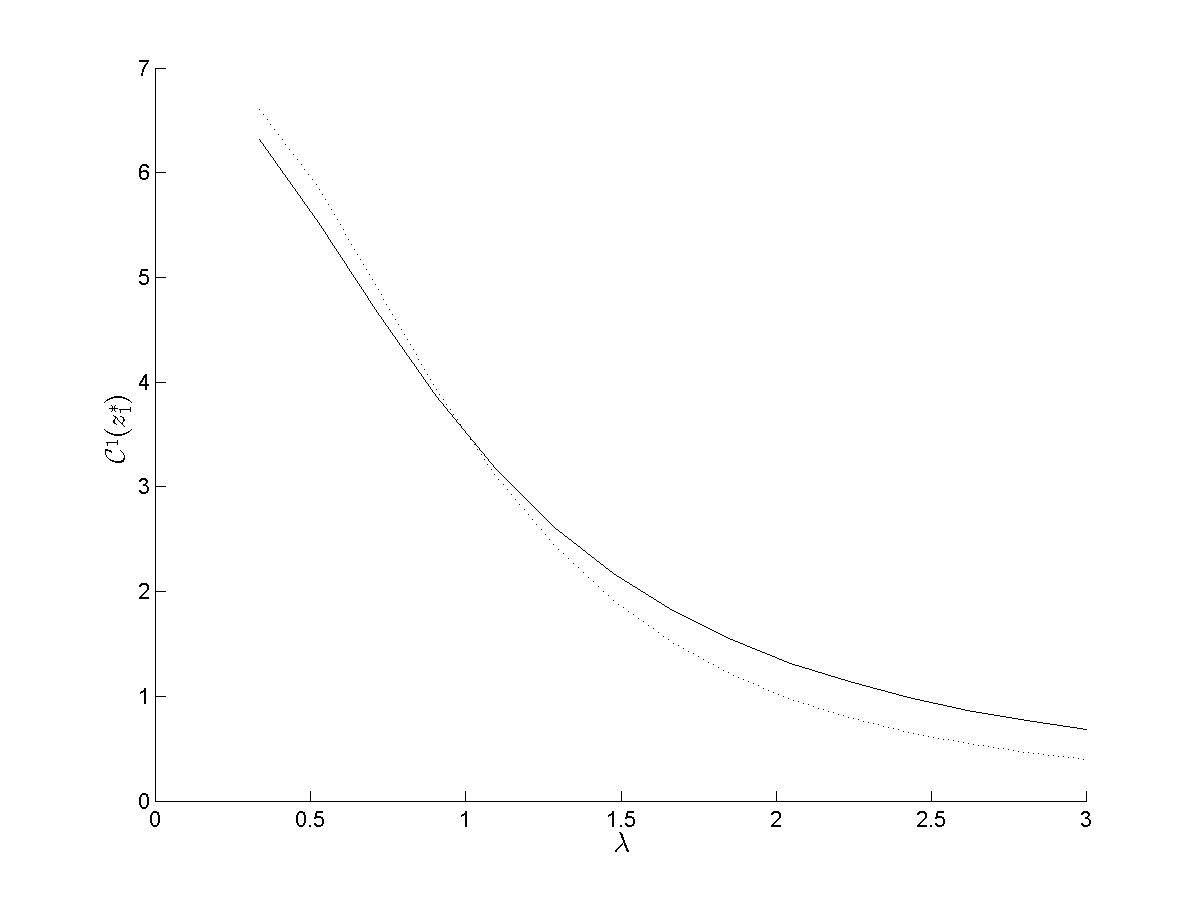
\includegraphics[scale=0.5]{Matlab/PrivateInformation/Plots/StaticPIConsumptionPlan.png}

	\caption{The plot depicts consumption of Agent 1 in $t=1$, state $z_1$. The dotted line is the benchmark without concerns for model ambiguity.}
	\label{fig:BondEconomyOucomes}
\end{figure} 
\subsection{Dynamic Incentives - I}
The previous section assumed private information only in $t=1$. This simplified the set of inecentive inequalities in \ref{tab:StaticICIneq} to a single equality constraint \ref{eq:StaticIC}. In a more dynamic setting these constraints are `occasionally'' binding. In this section I will setup a two period version of this problem with an ex-ante recursive formulation. The planner now chooses a \emph{consumption menu} and a \emph{continuation plan} before the private information is revealed. In a way he can use both these levers to provide incentives. 

\section{Conclusion}

\appendix
\section{Sequential problem}
\section{Decentralized Competitive equilibrium}
\subsection{Agent-i's problem}
Given his endowment process $e^i(z)$ and initial assets $a^i(z)$, Agent $i$ takes the consumption-portfolio decision by solving the following problem
\[V^i(a^i(z),z,\pi)=\max_{a^i(z^*),c^i}\mathbb{T}^i_2\left[ u(c^i)+\delta\mathbb{T}_1\left[V^i(a^i(z^*),z^*,\pi^*)\right]\right]\]

s.t.

\[c^i+\sum_{z^*} q(z^* | z)a^i(z^*)=a^i(z)+e^i(z)\]

\subsection{Recursive Competitive Equilibrium}
\noindent Given the $\{e^i,a^i(z0)\}_{i\in\mathcal{I}}$ a Recursive Competitive Equilibrium(RCE) is $\{c^i,a^i(z^*)\}_{i \in \mathcal{I}}, q(z^*|z)$ such that both the agents solve their respective problems and asset markets clear i.e
\[\sum_{i \in \mathcal{I}}a^i(z^*)=0\]

\noindent The FOCs of the agent's problem imply the following expression for asset prices 
\[q(z^*|z)=\delta \left(\sum_{m \in M}\tilde{\pi}^i(m)\tilde{P^i}_z(z^* |z,m)\right)\frac{V^i_a[a^i(z^*),z^*,\pi^*]}{u'(c^i)}\]
Where
\[\tilde{P}^i  \propto P\exp\left\{\frac{-V^i[a^i(z^*),z^*,\pi^*]}{\theta^1}\right\}\]

\[\tilde{\pi}^i  \propto \pi \exp\left\{-\frac{ u^(c^i)+\delta \mathbb{T}^2 V^i[a^i(z^*),z^*,\pi^*] }{\theta^2}\right\} \]

Dividing the FOCs across agents we have,
\[\frac{u'(c)}{u'(y(z)-c)}=\frac{\left(\sum_{m \in M}\tilde{\pi}^i(m)\tilde{P^i}_z(z^* |z,m)\right)}{\left(\sum_{m \in M}\tilde{\pi}^j(m)\tilde{P^j}_z(z^* |z,m)\right)}\left(\frac{V^i_a[a^i(z^*),z^*,\pi^*]}{V^j_a[a^j(z^*),z^*,\pi^*]}\right)\]
Comparing this to the Planner's FOC's
\begin{enumerate}
\item At the equilibrium,
\[\left(\frac{V^i_a[a^i(z^*),z^*,\pi^*]}{V^j_a[a^j(z^*),z^*,\pi^*]}\right)\approx \left.\frac{\frac{\partial V^1}{\partial a^1}(z^*)}{\frac{\partial V^2}{\partial a^2}(z^*)}\right |_{a^1(z^*)+a^2(z^*)=0}\]
or

\[\left.\frac{\partial V^1}{\partial V^2}(z^*)\frac{\partial a^2}{\partial a^1}(z^*)\right |_{a^1(z^*)+a^2(z^*)=0}=-\frac{\partial V^1}{\partial V^2}(z^*)=\textbf{$\mathcal{Q}_v(z^*)$}\]
\item $\frac{u'(c)}{u'(y-c)}=\lambda $

\end{enumerate}
\emph{Thus the Planner's problem solves the RCE with the following choice for asset prices}

\[q(z^* |z )=\delta \left(\sum_{m \in M}\tilde{\pi}^1(m)\tilde{P^1}_z(z^* |z,m)\right)\frac{ u'(c^*)}{u'(c)}\]

\subsection{Wealth and Continuation values}
We can compute mapping that links the wealth shares and the contiuation values by solving the following functional equation. Let $\mathcal{A}(v,z,\pi)$ be the wealth of Agent 1 corresponding to initial promised value of Agent 2 -v in the state $(z,\pi)$. 
\begin{equation}
c(v,z,\pi) +\sum_{z^*} {q(z^*|v,z,\pi) \mathcal{A}(z^*,\pi^*[\pi],v^*[v,z,\pi])}=\mathcal{A}(v,z,\pi)+y(z)s(z)
\end{equation}
Where the functions $c,v^*$ solve the Planners problem and $q$ are corresponding shadow prices for the decentralized equilibrium.

%\begin{lemma}
%\label{lemma-3}
%Bayes rule implies that 
%\[\pi^*[m^*|z^*,z,\pi]\propto \sum_{m}P_M[m^*|m]P_Y[y^*|y,m]P_{S|Y}[s^*|y^*,m]\]
%When the model space is complete we can decompose $P_M$ into $P_{\alpha}$ and $P_{\beta}$ such that
%\[P_M[m^*|m]=P_{\alpha}[\alpha(m^*)|\alpha(m)]P_{\beta}[\beta(m^*)|\beta(m)]\]
%Thus we have
%\[\pi^*[m^*|z^*,z,\pi]\propto \sum_{m}P_\alpha[\alpha(m^*)|\alpha(m)]P_Y[y^*|y,\alpha(m)]P_\alpha[\beta(m^*)|\beta(m)]P_{S|Y}[s^*|y^*,\beta(m)]\]
%Using the deifinition of $\pi^*[\alpha^*]$ we have
%\[\sum_{m^* \in \mathcal{\alpha(m^*)}}\pi^*[m^*|z^*,z,\pi]\propto \sum_{m^* \in \mathcal{\alpha(m^*)}} \sum_{m}P_\alpha[\alpha(m^*)|\alpha(m)]P_Y[y^*|y,\alpha(m)]P_\alpha[\beta(m^*)|\beta(m)]P_{S|Y}[s^*|y^*,\beta(m)]\]
%Since $\mathcal{\alpha(m^*)}$ is independent of $\alpha(m^*)$ we can split the sum into ``$\alpha$'' and ``$\beta$'' components
%\pi^*[\alpha(m^*)]\propto \left( \sum_{m}P_\alpha[\alpha(m^*)|\alpha(m)]P_Y[y^*|y,\alpha(m)]\right)\left(\sum_{\mahcal{M}}P_\alpha[\beta(m^*)|\beta(m)]P_{S|Y}[s^*|y^*,\beta(m)]\right)\]
%Since the last bracket term is independent of $\alpha(m^*)$ we can drop it from the constant of propotionality
%\end{lemma}
%\textbf{Proposition : 5}
%\begin{proof}
%We need to verify that the restrictions on the policy rules are consistent with the FOC of the Planners problem. 
%
%First note that $\pi^*$ and consumption being dependent only on the realization of the aggregate shock implies that $\mathcal{Q}$ inherits the same property. \footnote{This can be verified by iterating $\mathcal{Q} = \mathbb{T}^2_{\theta_2} u[c(y)]+\delta \mathbb{T}^1_{\theta_1,m} Q^*$ using the restrictions on $c,v^*$}
%
%\[\mathcal{Q}(v,z,\pi)=\mathcal Q(v,z',\pi')\]
%
%Since $y(z^*)=y(z^{**})$ and we have $v^*(z^*)=v^*(z^{**})$ the value for Agent 1 in the next period will also satisfy 
%\[c(z^*,\pi^*,v^*)=c(z^{**},\pi^{**},v^{**})\]
%\[\mathcal{Q}[z^*,\pi^*,v^*]=\mathcal{Q}[z^{**},\pi^{**},v^{**}]\]
%
%Let $V^1(z^*)=Q(z^*,\pi^*,v^*)$ and $V^2(z^*)=v^*(z^*)$
%
%Since $\lambda[z^*]=\lambda[z^{**}]$ the Planners FOC implies that
%\[\left(\frac{\sum_{m}\tilde \pi^i(m)\tilde P^i(z^*|z)}{\sum_{m}\tilde \pi^i(m)\tilde P^i(z^{**}|z)}\right)\] is independent of $i$
%
%We can write $\tilde{\pi}^i(m)$ as 
%\begin{subequations}
%\label{tilde-pi-i}
%\begin{align}
% \tilde{\pi}^i(m)&=\frac{\pi(m) \exp\left\{-\frac{1}{\theta_2}\left[u(c^i)+\delta\mathbb{T}^1_{\theta_1,m}V^i(Z^*)\right]\right\}}{\sum_{m}{\pi(m) \exp\left\{-\frac{1}{\theta_2}\left[u(c^i)+\delta\mathbb{T}^1_{\theta_1,m}V^i(Z^*)\right]\right\}}}\\
%&=\frac{\pi(m) \exp\left\{-\frac{1}{\theta_2}\left[\delta\mathbb{T}^1_{\theta_1,m}V^i(Z^*)\right]\right\}}{\sum_{m}{\pi(m) \exp\left\{-\frac{1}{\theta_2}\left[\delta\mathbb{T}^1_{\theta_1,m}V^i(Z^*)\right]\right\}}}\\
%&=	\frac{\pi(m) \left(\exp\left \{\mathbb{T}^1_{\theta_1,m}V^i(Z^*)\right\}\right)^{^{\frac{-\delta}{\theta_2}}}}{\sum_{m}{\pi(m) \exp\left\{-\frac{1}{\theta_2}\left[\delta\mathbb{T}^1_{\theta_1,m}V^i(Z^*)\right]\right\}}}
%\end{align}
%\end{subequations}
%\begin{subequations}
%\label{tilde-p-i}
%Further we can write $\tilde{P}_{Z}^{i}(z^*|z,m)$ as
%\begin{align}
%\tilde{P}_{Z}^{i}(z^*|z,m)&=\frac{P_Z(z^*|z,m)\exp\left\{-\frac{1}{\theta_1} V^i(z^*)\right\}}{\sum_{z^*}{P_Z(z^*|z,m)\exp\left\{-\frac{1}{\theta_1} V^i(z^*)\right \}}}\\
%&==\frac{P_Z(z^*|z,m)\exp\left\{-\frac{1}{\theta_1} V^i(z^*)\right\}}{\left(\exp\left\{ \mathbb{T}^1_{\theta_1,m}V^i(Z^*)\right\}\right)^{-\frac{1}{\theta_1}}}
%\end{align}
%\end{subequations}
%
%Multipying $\ref{tilde-pi-i}$ and $\ref{tilde-p-i}$ and summing over $m$ we have 
%
%\[\sum_{m}\tilde \pi^i(m)\tilde P^i(z^*|z)=\left(\frac{\exp\left\{-\frac{1}{\theta_1} V^i(z^*)\right\}}{\sum_{m}{\pi(m) \exp\left\{-\frac{1}{\theta_2}\left[\delta\mathbb{T}^1_{\theta_1,m}V^i(Z^*)\right]\right\}}}\right)\left(\sum_{m}\pi(m)P_Z(z^*|z,m)\left(\exp\left \{\mathbb{T}^1_{\theta_1,m}V^i(Z^*)\right\}\right)^{\left(\frac{\theta_1-\delta\theta_2}{\theta_1\theta_2}\right)}\right)\]
%
%
%Computing the above expression for $z^*$ and $z^{**}$ we have
%\begin{equation}
%\label{ratio-lambdastar}
%\left(\exp\left\{\frac{V^i(z^{**})-V^i(z^*)}{\theta_1}\right\}\right)
%\frac{\sum_{m}\pi(m)P_Z(z^*|z,m)
%\left(\exp\left \{
%\mathbb{T}^1_{\theta_1,m}V^i(Z^*)
%\right\}
%\right)^{\left(\frac{\theta_1-\delta\theta_2}{\theta_1\theta_2}\right)}
%}
%{\sum_{m}\pi(m)P_Z(z^{**}|z,m)
%\left(
%\exp\left \{
%\mathbb{T}^1_{\theta_1,m}V^i(Z^*)
%\right\}
%\right)^{\left(\frac{\theta_1-\delta\theta_2}{\theta_1\theta_2}\right)
%}
%}
%\end{equation}
%
%
%Define $F_{m}^i$
%\[F_{m}^i=\left(\exp\left \{
%\mathbb{T}^1_{\theta_1,m}V^i[y(z^*)]
%\right\}
%\right)^{\left(\frac{\theta_1-\delta\theta_2}{\theta_1\theta_2}\right)}
%\]
%
%Rewriting $\ref{ratio-lambdastar}$ with $F^i_{m}$ we have
%\begin{equation}
%\label{ratio-lambdastar-2}
%\frac{\sum_{m}\pi(m)P_Z(z^*|z,m)F^i_m
%}
%{\sum_{m}\pi(m)P_Z(z^*|z,m)F^i_m
%}
%\end{equation}
%
%We need to check that $\ref{ratio-lambdastar-2}$ is independent of $i$. 
%\begin{enumerate}
%	\item When  $\delta\theta_1=\theta2$, we have $F^i_m=1$ so $\ref{ratio-lambdastar-2}$ is independent of $i$
%%	\item When $s$ and $y$ are independent and $\mathcal{M}$ is complete we can write the ratio as
%%	\begin{align}
%%&=\frac{
%%\sum_{\alpha_m}\sum_{\beta_m}\pi(\alpha_m)\pi(\beta_m)P_Z(s^*|s,\beta_m)P_Z(\bar{y}|y,\alpha_m)F^i_{\alpha_m
%%}
%%}
%%{\sum_{\alpha_m}\sum_{\beta_m}\pi(\alpha_m)\pi(\beta_m)P_Z(s^{**}|s,\beta_m)P_Z(\bar{y}|y,\alpha_m)F^i_{\alpha_m
%%}
%%}\\
%%&=\frac{
%%\left(\sum_{\alpha_m}\pi(\alpha_m)P_Z(\bar{y}|y,\alpha_m)F^i_{\alpha_m
%%}\right)\left(\sum_{\beta_m} \pi(\beta_m)P_Z(s^*|s,\beta_m)\right)
%%}
%%{
%%\left(\sum_{\alpha_m}\pi(\alpha_m)P_Z(\bar{y}|y,\alpha_m)F^i_{\alpha_m
%%}\right)\left(\sum_{\beta_m} \pi(\beta_m)P_Z(s^{**}|s,\beta_m)\right)
%%}\\
%%&=\frac{
%%\left(\sum_{\beta_m} \pi(\beta_m)P_Z(s^*|s,\beta_m)\right)
%%}
%%{
%%\left(\sum_{\beta_m} \pi(\beta_m)P_Z(s^{**}|s,\beta_m)\right)
%%}
%%\end{align}
%%which is indepedent of $i$
%\item Further if  $P_M(s^*|y^*,z,m)=\bar{\beta} \quad \forall m s.t \pi(m) >0$   
%\begin{align}
%&=\frac{\sum_{m}\pi(m)P_Z(s^*|\bar{y},z)P_Z(\bar{y}|z)F^i_m
%}
%{\sum_{m}\pi(m)P_Z(s^{**}|\bar{y},z)P_Z(\bar{y}|z)F^i_m
%}\\
%&=\frac{P_Z(s^*|\bar{y},z)}
%{
%P_Z(s^*|\bar{y},z)
%}
%\end{align}
%
%\item Finally if $\mathcal{M}_{\alpha}=1$, the term $F^i_m$ is independent of $m$ and drops out 
%
%\end{enumerate}
%
%If $\pi^*_{\alpha}$ depends on $s^*$ then 
%\[\mathcal{Q}[z^*,\pi^*,v^*] \neq \mathcal{Q}[z^{**},\pi^{**},v^{**}]\] as long as $Q_{\pi} > 0$
%\end{proof}
%
%\section{Stability}
%
%Since the learning process does not converge to a degenerate distribution, I expect that $\lambda^{*}$ and $V^{*}$ also inherit these properties. Consider the following example - Compute the utility consequence of the plan in which each agent consumes half of the aggregate endowment.  This is a natural way to construct a steady state as there is no other source of heterogenity except initial promised values. 


\section{Other Proofs}






\begin{proof}
The FOC imply $\mathcal{C}^1(\lambda)$ such that
\begin{equation}
\frac{\tilde{\beta}^1(z)u_{c}[c]-\tilde{\beta}^2(z)\lambda u_{c}[y-c)]}{ (1-\tilde{\beta^1}(z))u_{c}[c+\Delta]-\lambda (1-\tilde{\beta^2}(z))u_{c}[y-c-\Delta]}=-1
\label{eq:c1lambda}
\end{equation}

Further $\mathcal{C}^1_{\infty}$ solves
\begin{equation}
\frac{u_{c}[c]-\lambda u_{c}[y-c]}{ u_{c}[c+\Delta]-\lambda u_{c}[y-c-\Delta]}=-\frac{1-\beta(z)}{\beta(z)}
\label{eq:c1EUlambda}
\end{equation}

Now $\bar{\lambda}$ is such that $C^{1}_{\infty}(\bar{\lambda})=C^{1}(\bar{\lambda})$

Using $\ref{eq:c1lambda}$ and \ref{eq:c1EUlambda} $\bar{\lambda}$ will satisfy
\begin{equation}
\frac{\tilde{\beta}^1(z)u_{c}[\mathcal{C}^1_{\infty}(\bar{\lambda})]-\tilde{\beta}^2(z)\lambda u_{c}[y-\mathcal{C}^1_{\infty}(\bar{\lambda})]}{ (1-\tilde{\beta^1(z)})u_{c}[\mathcal{C}^1_{\infty}(\bar{\lambda})+\Delta]-\bar{\lambda} (1-\tilde{\beta^2(z)})u_{c}[y-\mathcal{C}^1_{\infty}(\bar{\lambda})-\Delta]}=-1
\end{equation}


Let 
\begin{align}
F^1(c)&=u_c(c)-u_c(c+\Delta)\\
F^2(c)&=u_c(y-c-\Delta)-u_c(y-c)
\end{align}

This implies
\begin{equation}
(\tilde{\beta}^1(z)-\beta) F^1[\mathcal{C}^1_{\infty}(\bar{\lambda})]+\bar{\lambda}(\tilde{\beta}^2(z)-\beta)F^2(\mathcal{C}^1_{\infty}(\bar{\lambda}))=0
\label{eq:barlambda}
\end{equation}
Define $\chi(\lambda)$ as the residual for the equation \ref{eq:barlambda}
\begin{equation}
(\tilde{\beta}^1(z)-\beta) F^1[\mathcal{C}^1_{\infty}(\lambda)]+\lambda(\tilde{\beta}^2(z)-\beta)F^2[\mathcal{C}^1_{\infty}(\lambda)]=\chi(\lambda)
\end{equation}


Note that,

\[\lim_{c\to 0} F^1(c) = \lim_{c \to 0}\left[\frac{u_c(c)-u_c(c+\Delta)}{c}c\right] = -u_{c,c}[\Delta] [\lim_{c \to 0} c]=0\]
\[\lim_{c\to y-\Delta} F^1(c) = \left[{u_c(c y-\Delta)-u_c(y)}\right] \approx -\Delta u_{c,c} [y] > 0\]
\[\lim_{c\to y-\Delta} F^2(c) = 0\]


Since $\frac{\partial \mathcal{C}^1_{\infty} (\lambda)}{\partial \lambda} <0 $, we have

\[\text{sgn} \chi(\infty) = \text{sgn} (\tilde{\beta}^2(z)-\beta)\]
\[\text{sgn} \chi(0) = \text{sgn} (\tilde{\beta}^1(z)-\beta)\]

Since $\tilde {\beta} ^1(1) > \beta > \tilde{\beta}^2(1)$ and the opposite for $z=2$ , there exists a $\bar{\lambda}$ such that
\[\chi(\bar{\lambda})=0\]
Define $c^{M}=\frac{y-\Delta}{2}$. We have
\begin{equation}
c^M=y-c^M-\Delta
\nonumber
\end{equation}

$c=c^M$ and $\beta=\frac{1}{2}$ imply that
\begin{enumerate}
	\item $\bar{c}(1)=c^M$ 
	\item $F^1(c^M)=F^2(c^M)$
	\item $\tilde{\beta}^1+\tilde{\beta}^2=1$
\end{enumerate}

From eq \ref{eq:barlambda} we have that $\bar{\lambda}$ is pinned down by
\[
(\tilde{\beta}^1-\beta) F^1[\bar{c}(\bar{\lambda})]+\bar{\lambda}(\tilde{\beta}^2-\beta)F^2(\bar{c}(\bar{\lambda}))=0
\]
\[F(c^M)(\tilde{\beta}^1+\tilde{\beta}^2-1)=0\]
\begin{align*}
\tilde{\beta}^1=\frac{\beta \exp \left\{ -\frac{u[c]}{\theta}\right\}}{\beta \exp \left\{ -\frac{u[c]}{\theta}\right\}+ (1-\beta)\exp \left\{ -\frac{u[y-c]}{\theta}\right\}}\\
\tilde{\beta}^2=\frac{\beta \exp \left\{ -\frac{u[y-c]}{\theta}\right\}}{\beta \exp \left\{ -\frac{u[y-c]}{\theta}\right\}+ (1-\beta)\exp \left\{ -\frac{u[y-c-\Delta]}{\theta}\right\}}
\end{align*}
At $c=c^M$ and $\beta=\frac{1}{2}$ we have
\begin{equation}
\tilde{\beta}^1+\tilde{\beta}^2=\frac{ \exp \left\{ -\frac{u[c^M]}{\theta}\right\}+ \exp \left\{ -\frac{u[y-c^M]}{\theta}\right\}}{ \exp \left\{ -\frac{u[y-c^M]}{\theta}\right\}+ \exp \left\{ -\frac{u[c^M]}{\theta}\right\}}
\end{equation}
or
\[\tilde{\beta}^1+\tilde{\beta}^2=1\]
\end{proof}
%
%\begin{enumerate}
%\item The composition of T1 and T2 is an contraction.
%\item Planners problem and complete markets (*)
%\item Concavity of value function
%\item Stability
%\item Log-homotheticity implications
%\item Survival examples
%\end{enumerate}
% \section{To Do}
% 
%\begin{enumerate}
%	\item REvise the consumption section. Draw only $\alpha(z^*|z,v)$ for $z^*$ such that $y(z^*)=y_l$ or $y(z^*)=y_h$. With this I can have IID,NonIID and Learning in the same graph.
%	\item Comment about the assymtery in slopes with respect to $v$ for difference $y(z^*)$
%	\item Think about the fact that the optimization fails at low $v$. We are evaluating the value function outside its domain of approximation. 
%	\item In the Learning case use exitflags to initialize only the correct points
%	\item In general come up with a strategy to solve this issue of how to solve the value function at the extremes
%	\item In the conclusion set up the future task as dealing with how other forms of heterogenity  - approximating model, ambiguity conscerns etc interact with market incompleteness.
%	\item  1 What do you mean by Knigtian uncertainty - Agents possibly entertaint more than one probablity specification for the randomness in the world. To complete a description of how agents behave in this setting we must specify a theory of how they deal with this multiplicity. Most models of ambiguity try to recast the decision making problem by positing a prioir selection rule confirming certain behavioral regularities.
%
%\end{enumerate}
\section{TO DO}
%\begin{enumerate}
%	\item Re-paramterize $P_Y$ such that the benchmark MPR=1 for all $\pi$. Now see what happens with ambiguity
%	\item Do a minimally stochastic case for complete markets
%\item Connect to Lasrs Lochter's paper
%\end{enumerate}
\end{document}